掌握数据结构对开发者来说很有必要,大多数时候存储数据的方式决定了应用程序的效率。以电子邮件客户端为例,你可以设计一个电子邮件客户端,显示最近10封电子邮件,用户在使用你的应用两年内会收到数十万封电子邮件。当用户需要搜索电子邮件时,数据结构就会发挥重要作用。你储存成千上万封电子邮件的方式,排序和搜索它们的方法(算法)则非常重要。 \par
开发者在项目中努力寻找日常问题的最佳解决方案,使用经过验证的数据结构和算法可以极大地改善工作效率。好的程序最重要的特点是速度,我们可以通过设计新的算法,或使用现有的算法来得到良好的运行速度。 \par
C++20引入了元类型的概念——描述其他类型的类型,这个强大特性使数据架构更加完整。 \par
C++标准模板库(STL)中包含了大量的数据结构和算法。我们将探索利用STL容器来使用数据结构有效地组织数据的方法,然后将深入研究STL提供的算法实现。理解和使用STL容器中的概念至关重要,因为C++20通过引入迭代器概念,对迭代器进行了重大改进。 \par
本章中,我们将了解以下内容: \par

\begin{itemize}
	\item 数据结构
	\item STL容器
	\item 概念和迭代器
	\item 主流算法
	\item 探索树和图
\end{itemize}

\noindent\textbf{}\ \par
\textbf{编译器要求} \ \par
g++编译器需要添加编译选项 \texttt{-std=c++2a} 来编译本章的代码。可以从这里获取本章的源码文件:https:/​/github.​com/PacktPublishing/Expert-CPP \par

\noindent\textbf{}\ \par
\textbf{数据结构} \ \par
开发者可能很熟悉使用数组来存储和排序数据,也会在项目中大量使用数据结构,而不是数组。了解和应用正确的数据结构可能在程序性能中扮演着重要的角色。为了选择正确的数据结构,就需要更好地了解它们。一个明显的问题可能会出现:我们是否需要研究数据结构的集合——向量、链表、哈希表、图、树等。为了回答这个问题,让我们想象一个场景,在这个场景中,合适的数据结构的必要性将很明显地显现出来。 \par
之前介绍中,我们提到了设计电子邮件客户端,大致的了解一下它的设计和实现。 \par
电子邮件客户端是列出不同发件人邮件的应用。我们可以在台式电脑或智能手机上安装它,或者使用浏览器版本。电子邮件客户端应用的主要任务包括发送和接收电子邮件。现在假设我们正在设计简单的电子邮件客户机,假设我们使用一些库来封装发送和接收电子邮件的工作,这让我们更专注于设计专门用于存储和检索电子邮件的机制。客户端用户能够查看驻留在收件箱的邮件列表,还应该考虑用户可能想要对电子邮件执行的操作。他们可以一个个的删除,或者一次性删除很多,也可以随机选择任何一封邮件,回复发件人或转发给其他人。 \par
我们将在第10章中讨论软件设计过程和最佳实践。现在,让我们构建一个简单的Email对象,如下所示: \par

\begin{lstlisting}[caption={}]
struct Email
{
	std::string subject;
	std::string body;
	std::string from;
	std::chrono::time_point datetime;
};
\end{lstlisting}

第一件困扰我们的事情是将一组电子邮件存储容易访问的结构中,数组听起来可能不错。假设我们将所有收到的电子邮件存储在一个数组中,如下面的代码块所示: \par

\begin{lstlisting}[caption={}]
// let's suppose a million emails is the max for anyone
const int MAX_EMAILS = 1'000'000;
Email inbox[MAX_EMAILS];
\end{lstlisting}

我们可以以任何形式存储10封电子邮件——这不会影响应用的性能。然而,随着时间的推移,电子邮件的数量会增长。对于新收到的电子邮件,将带有相应字段的Email对象推送到inbox数组中,数组的最后一个元素表示最近收到的电子邮件。因此,要显示最近10封电子邮件的列表,需要读取并返回数组的最后10个元素。 \par
当试图操作存储在inbox数组中的数千封电子邮件时,问题就出现了。如果想在所有的电子邮件中搜索“friend”这个词,就必须扫描数组中的所有电子邮件,并在单独的数组中收集包含单词friend的电子邮件: \par

\begin{lstlisting}[caption={}]
std::vector<Email> search(const std::string& word) {
	std::vector<Email> search_results;
	for (all-million-emails) {
		if (inbox[i].subject.contains(word)) {
			search_results.push_back(inbox[i]);
		}
	}
	return search_results;
}
\end{lstlisting}

对于小型集合来说,使用数组存储数据绰绰有余。处理更大数据集的应用中,这种情况会变得复杂。使用特定数据结构的目的是使应用运行得更流畅。前面的示例展示了一个简单的问题:搜索电子邮件列表以匹配特定的值。在电子邮件中进行查找时,需要在合理的时间范围内。 \par
如果假设电子邮件的主题可能包含最多10个单词,那么搜索电子邮件主题中的特定单词需要将该单词与主题中的所有单词进行比较。最坏的情况下,没有任何匹配。强调最坏的情况,是因为只有在这种情况下的查找,才需要检查主题中的每个单词。对成千上万的电子邮件执行同样的操作,会让用户等的不耐烦。 \par
就应用程序效率而言,为特定问题选择正确的数据结构至关重要,例如:假设使用哈希表将单词映射到Email对象,每个单词都将映射到包含该单词的电子邮件对象列表。这种方法将提高搜索操作的效率,如下图所示:\par

\begin{center}
	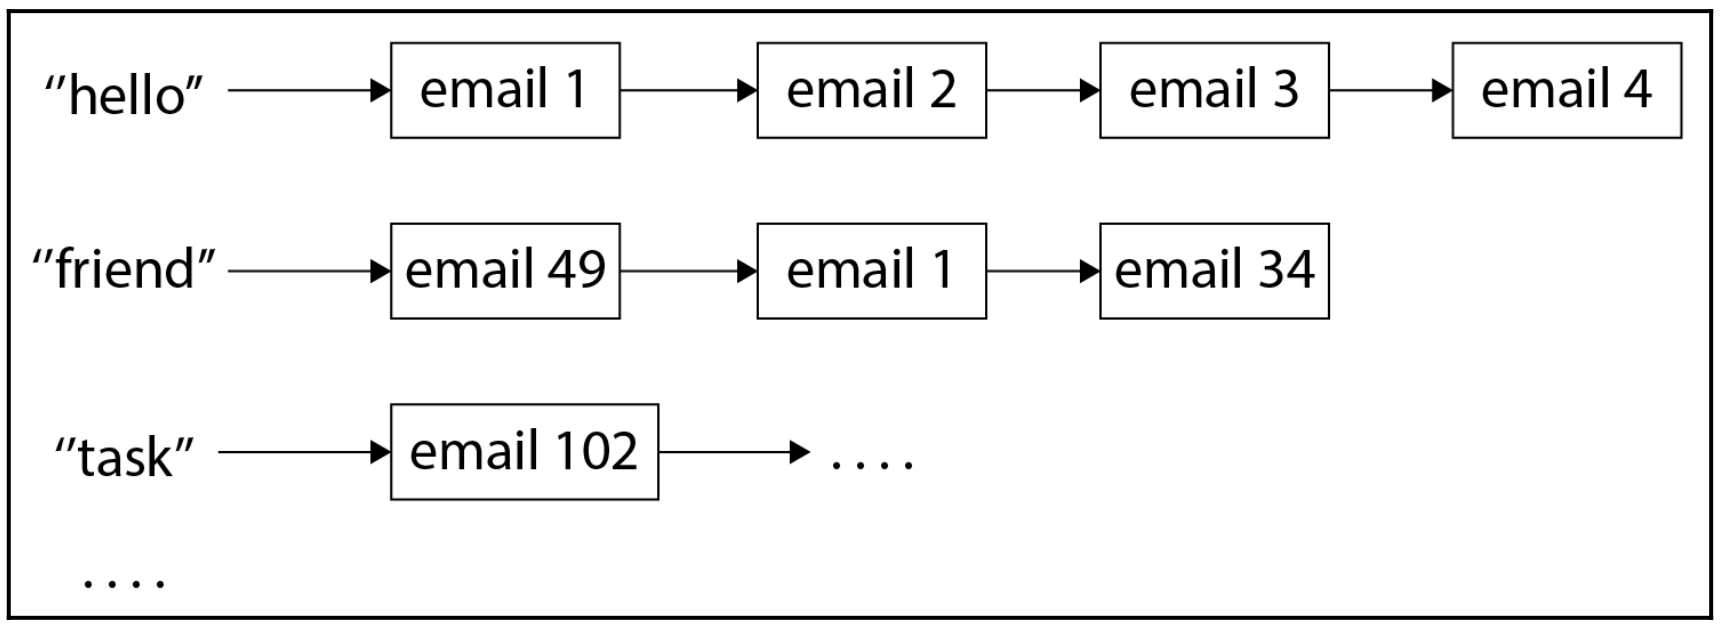
\includegraphics[width=0.6\textwidth]{content/Section-2/Chapter-6/1}
\end{center}

search()函数只返回哈希表键所指向的列表: \par

\begin{lstlisting}[caption={}]
std::vector<Email> search(const std::string& word) {
	return table[word];
}
\end{lstlisting}

这种方法只需要处理每个收到的电子邮件,将其拆分为单词并更新哈希表。 \par

\hspace*{\fill} \\ %插入空行

\includegraphics[width=0.05\textwidth]{images/tip}
简单起见,直接使用Email对象,而不是引用。请注意,最好将指向电子邮件的指针存储在vector中。 \par
\noindent\textbf{}\ \par

现在,让我们看看不同的数据结构及其应用。 \par

\noindent\textbf{}\ \par
\textbf{连续的数据结构} \ \par
开发人员使用的最常见数据结构是动态增长的一维数组——vector。STL提供了一个相同名称的容器:std::vector。vector的关键思想是,包含按顺序放置在内存中的相同类型的项。例如,由4个字节整数组成的向量,将具有如下的内存布局。每个框代表一个4字节的空间。向量的下标在下图的右侧: \par

\begin{center}
	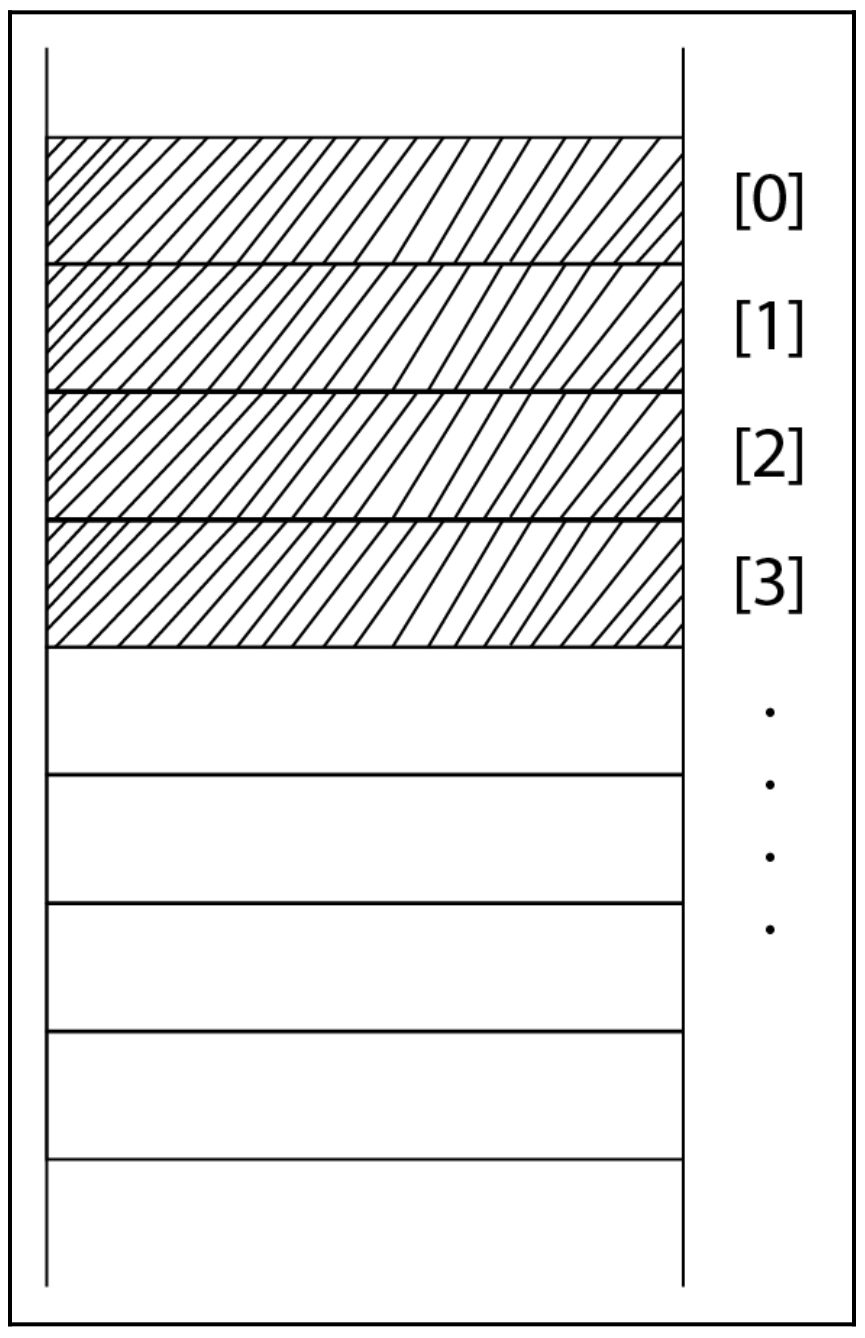
\includegraphics[width=0.4\textwidth]{content/Section-2/Chapter-6/2}
\end{center}

vector的物理结构允许实时访问它的任何元素。 \par

\hspace*{\fill} \\ %插入空行

\includegraphics[width=0.05\textwidth]{images/warn}
我们应该区分容器和操作,以便在问题中正确地应用。为此,我们根据容器中元素的数量定义操作时间复杂度。例如,vector的元素访问可定义为常量时间操作,这意味着无论vector的长度如何,访问vector中的项都需要相同数量的指令。 \par
\noindent\textbf{}\ \par

访问vector的第一个元素和访问向量的第100个元素需要相同的工作量,这就称之为常数时间操作,也称为O(1)操作。 \par

虽然vector中的元素访问速度很快,但添加新元素有点棘手。当在vector的末尾插入一个新元素时,还应该考虑vector的容量。当没有更多的空间分配给vector时,它应该动态地增加大小。看看下面的Vector类及其push\underline{ }back()函数: \par

\begin{lstlisting}[caption={}]
template <typename T>
class Vector
{
public:
	Vector() : buffer_{nullptr}, capacity_{2}, size_{0}
	{
		buffer_ = new T[capacity_]; // initializing an empty array
	}
	~Vector() { delete [] buffer_; }
	// code omitted for brevity
public:
	void push_back(const T& item)
	{
		if (size_ == capacity_) {
			// resize
		}
		buffer_[size_++] = item;
	}
	// code omitted for brevity
};
\end{lstlisting}

深入研究push\underline{ }back()函数的实现之前,让我们先看看下图: \par

\begin{center}
	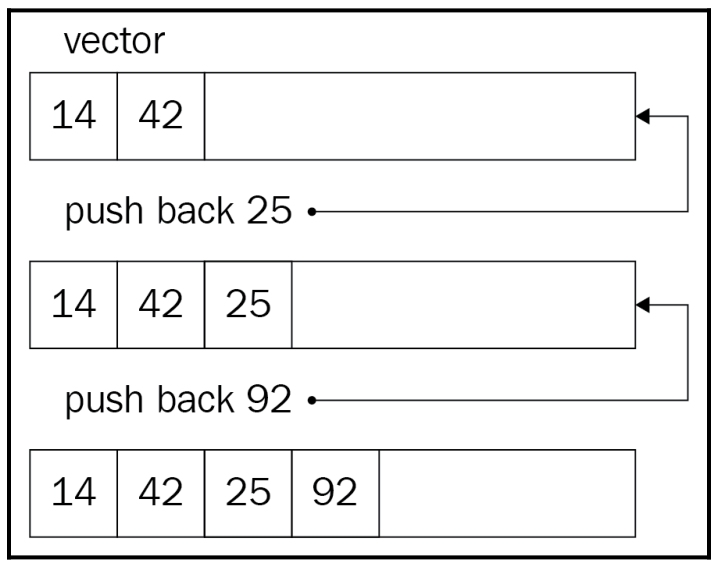
\includegraphics[width=0.6\textwidth]{content/Section-2/Chapter-6/3}
\end{center}

我们应该分配一个全新的数组,将旧数组的所有元素复制到新数组中,然后将新插入的元素添加到新数组末尾的下一个空闲槽中。如下面的代码片段所示: \par

\begin{lstlisting}[caption={}]
template <typename T>
class Vector
{
	public:
	// code omitted for brevity
	void push_back(const T& item)
	{
		if (size_ == capacity_) {
			capacity_ *= 2; // increase the capacity of the vector twice
			T* temp_buffer = new T[capacity_];
			// copy elements of the old into the new
			for (int ix = 0; ix < size_; ++ix) {
				temp_buffer[ix] = buffer_[ix];
			}
			delete [] buffer_; // free the old array
			buffer_ = temp_buffer; // point the buffer_ to the new array
		}
		buffer_[size_++] = item;
	}
	// code omitted for brevity
};
\end{lstlisting}

大小调整因子可以用不同的方式选择——我们将其设置为2,这将使vector在满载时,空间增长两倍。因此,我们坚持认为,大多数情况下,在向量的末尾插入一个新项需要常数时间。它只是在空闲槽添加项,并增加其私有size\underline{ }变量。有时,添加新元素需要分配一个新的、更大的vector,并需要将旧的vector复制到新的vector中。对于这样的情况,操作需要平摊常数时间才能完成。 \par
但当我们在vector前面加一个元素时就不能这么说了,所有其他元素都应该向右移动一个槽,以便为新元素腾出一个槽,如下图所示: \par

\begin{center}
	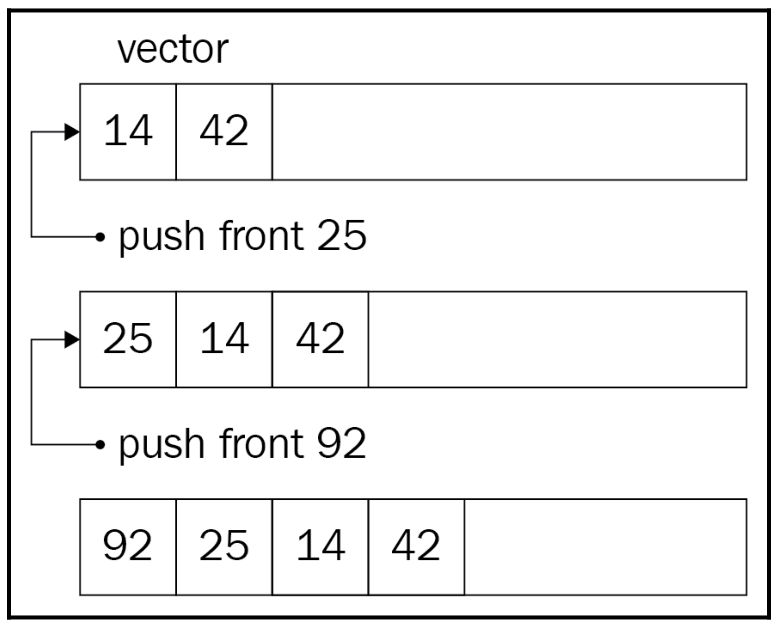
\includegraphics[width=0.6\textwidth]{content/Section-2/Chapter-6/4}
\end{center}

下面是我们如何在Vector类中实现它: \par

\begin{lstlisting}[caption={}]
// code omitted for brevity
void push_front(const T& item)
{
	if (size_ == capacity_) {
		// resizing code omitted for brevity
	}
	// shifting all the elements to the right
	for (int ix = size_ - 1; ix > 0; --ix) {
		buffer_[ix] = buffer[ix - 1];
	}
	// adding item at the front
	buffer_[0] = item;
	size_++;
}
\end{lstlisting}

在只需要在容器前端插入新元素的情况下,选择vector不是一个好的选择,这时需要考虑一下其他容器。 \par

\noindent\textbf{}\ \par
\textbf{节点式数据结构} \ \par
节点式的数据结构不需要连续的内存块。基于节点的数据结构为其元素分配节点,没有任何顺序——在内存中随机分布。我们将每个项目表示为一个节点,然后链接到其他节点的节点。 \par
最流行的、入门级的节点式的数据结构是链表。下面的图表可视化显示了双链表的结构: \par

\begin{center}
	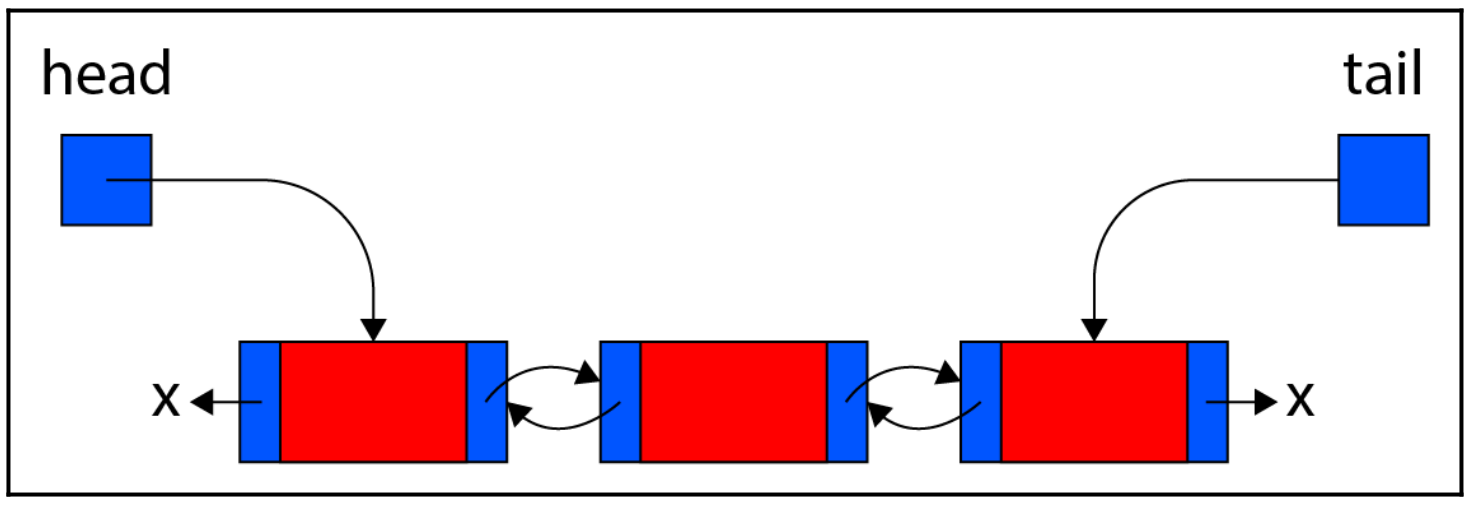
\includegraphics[width=0.6\textwidth]{content/Section-2/Chapter-6/5}
\end{center}

链表与向量有很大的不同。它的操作更快,但缺乏向量的紧凑性。 \par
为了保持简短,我们在列表的前面实现元素插入,将每个节点保持为一个结构体: \par

\begin{lstlisting}[caption={}]
template <typename T>
struct node
{
	node(const T& it) : item{it}, next{nullptr}, prev{nullptr} {}
	T item;
	node<T>* next;
	node<T>* prev;
};
\end{lstlisting}

请注意next成员——它指向同一个结构体,这种方式允许将节点链接在一起,如前面的示例所示。 \par
为了实现一个链表,需要一个指向它的第一个节点的指针,通常称为链表的头节点。在列表的前面插入一个元素很简单: \par

\begin{lstlisting}[caption={}]
template <typename T>
class LinkedList
{
	// code omitted for brevity
public:
	void push_front(const T& item)
	{
		node<T>* new_node = new node<T>{item};
		if (head_ != nullptr) {
			new_node->next = head_->next;
			if (head_->next != nullptr) {
				head_->next->prev = new_node;
			}
		}
		new_node->next = head_;
		head_ = new_node;
	}
private:
	node<T>* head_;
};
\end{lstlisting}

向列表中插入元素时,需要考虑以下三种情况: \par

\begin{itemize}
	\item 如前所述,在列表前面插入元素需要执行以下步骤: \par
	\begin{center}
		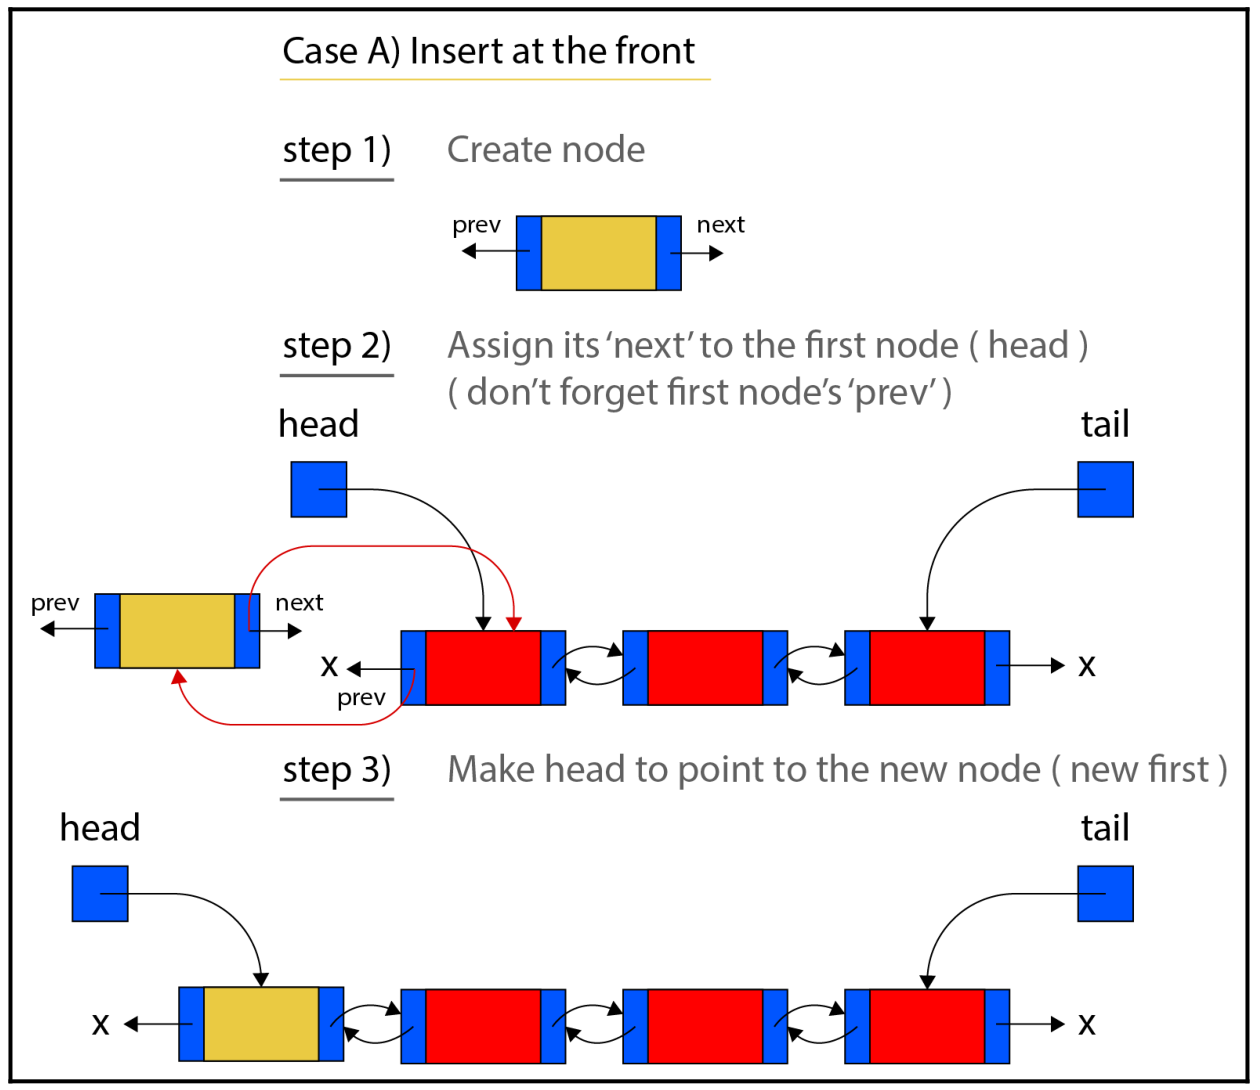
\includegraphics[width=0.6\textwidth]{content/Section-2/Chapter-6/6}
	\end{center}
	\item 在列表末尾插入一个元素,如下图所示: \par
	\begin{center}
		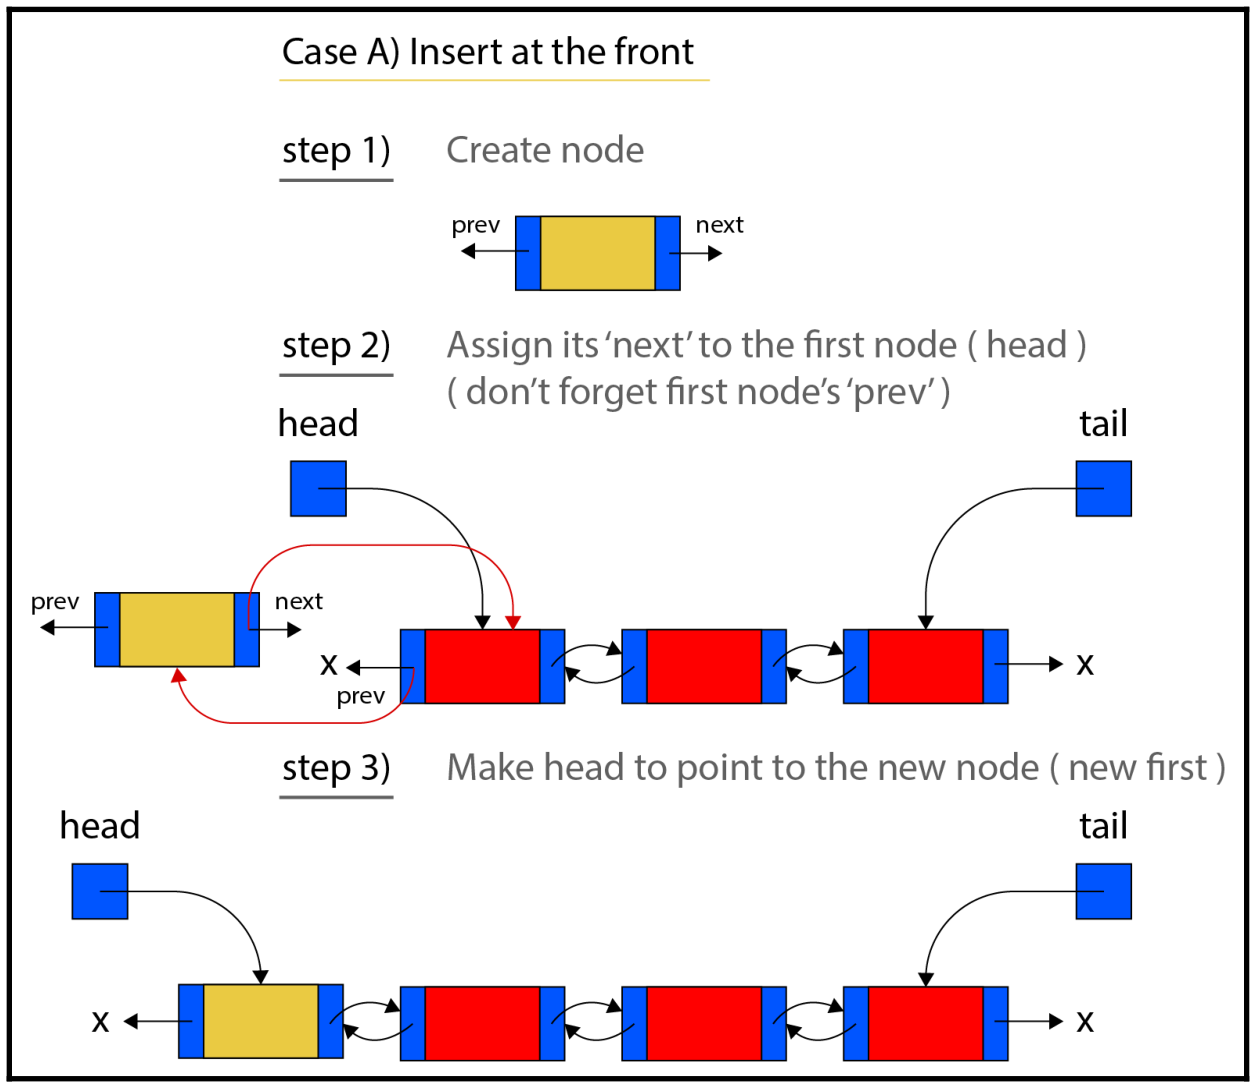
\includegraphics[width=0.6\textwidth]{content/Section-2/Chapter-6/7}
	\end{center}
	\item 最后,在列表中间插入一个元素的操作如下: \par
	\begin{center}
		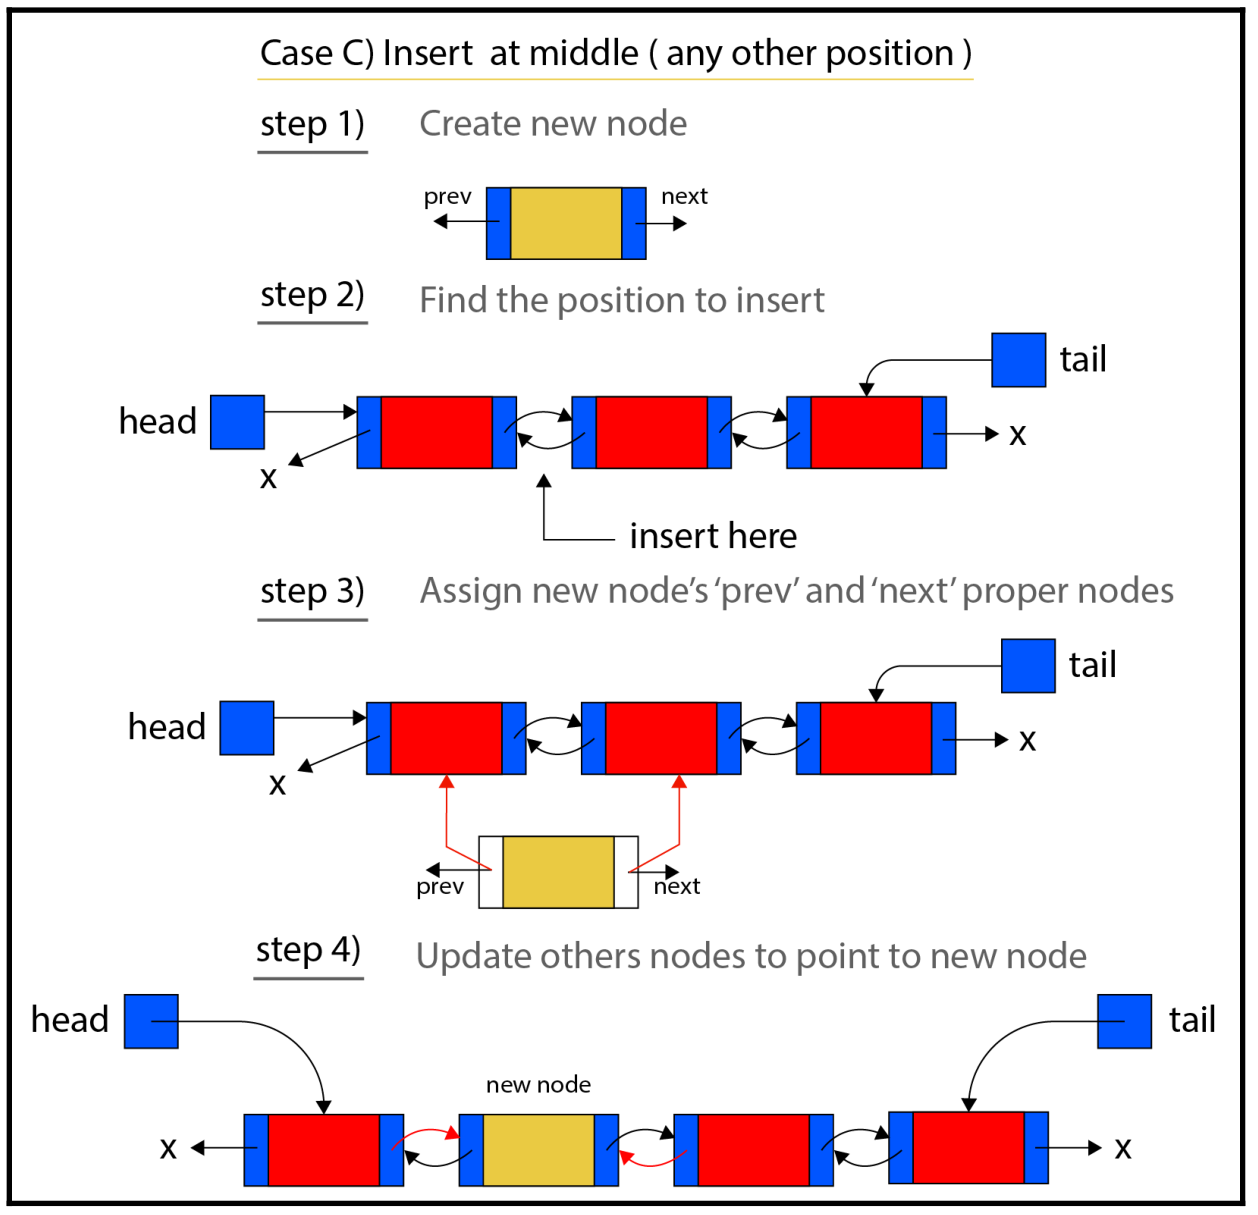
\includegraphics[width=0.6\textwidth]{content/Section-2/Chapter-6/8}
	\end{center}
\end{itemize}

向vector对象中插入元素与向list对象中插入元素明显不同。如何在vector和list中选择?应该专注行为和速度。例如,从vector中读取任何元素需要常量时间。我们可以在一个向量中存储100万封电子邮件,并且不需要任何额外的努力就可以检索位置为834,000的电子邮件。对于链表,操作是线性的。因此,如果需要存储主要用于读取而不是写入的数据集合,那么使用vector是更合理的选择。 \par
在列表的任何位置插入元素需要常量时间的操作,而vector将努力在随机位置插入元素。因此,当需要一个可以集中添加/删除数据的对象集合时,更好的选择是一个链表。 \par
我们还应该考虑缓存内存。向量具有良好的数据局部性,读取vector对象的第一个元素需要将前N个元素复制到缓存中。进一步读取vector元素会更快。对于链表,我们就不能这么说了。为了找出原因,让我们继续比较vector和链表的内存布局。 \par

\noindent\textbf{}\ \par
\textbf{容器的内存} \ \par
如前面的章节所示,对象会在进程的内存段上占用一定的内存空间。大多数时候,我们感兴趣的是堆栈或堆内存。自动对象占用堆栈空间,下面两个声明都在栈中: \par

\begin{lstlisting}[caption={}]
struct Email
{
	// code omitted for brevity
};
int main() {
	Email obj;
	Email* ptr;
}
\end{lstlisting}

虽然ptr表示指向Email对象的指针,但也在堆栈上占用空间。可以指向在堆上分配的内存位置,但指针本身(存储内存位置地址的变量)驻留在堆栈上。进一步使用向量和列表之前,理解和记住这一点非常重要。 \par
如本章前面所示,实现vector涉及到封装指向内部缓冲区的指针,该缓冲区代表指定类型的元素数组。声明Vector对象时,需要一定数量的堆栈内存来存储其成员数据。Vector类有以下三个成员: \par

\begin{lstlisting}[caption={}]
template <typename T>
class Vector
{
public:
	// code omitted for brevity
private:
	int capacity_;
	int size_;
	T* buffer_;
};
\end{lstlisting}

假设一个整数占用4个字节,一个指针占用8个字节,下面的Vector对象声明将占用至少16个字节的堆栈内存: \par

\begin{lstlisting}[caption={}]
int main()
{
	Vector<int> v;
}
\end{lstlisting}

下面是对前面代码的内存布局的描述: \par

\begin{center}
	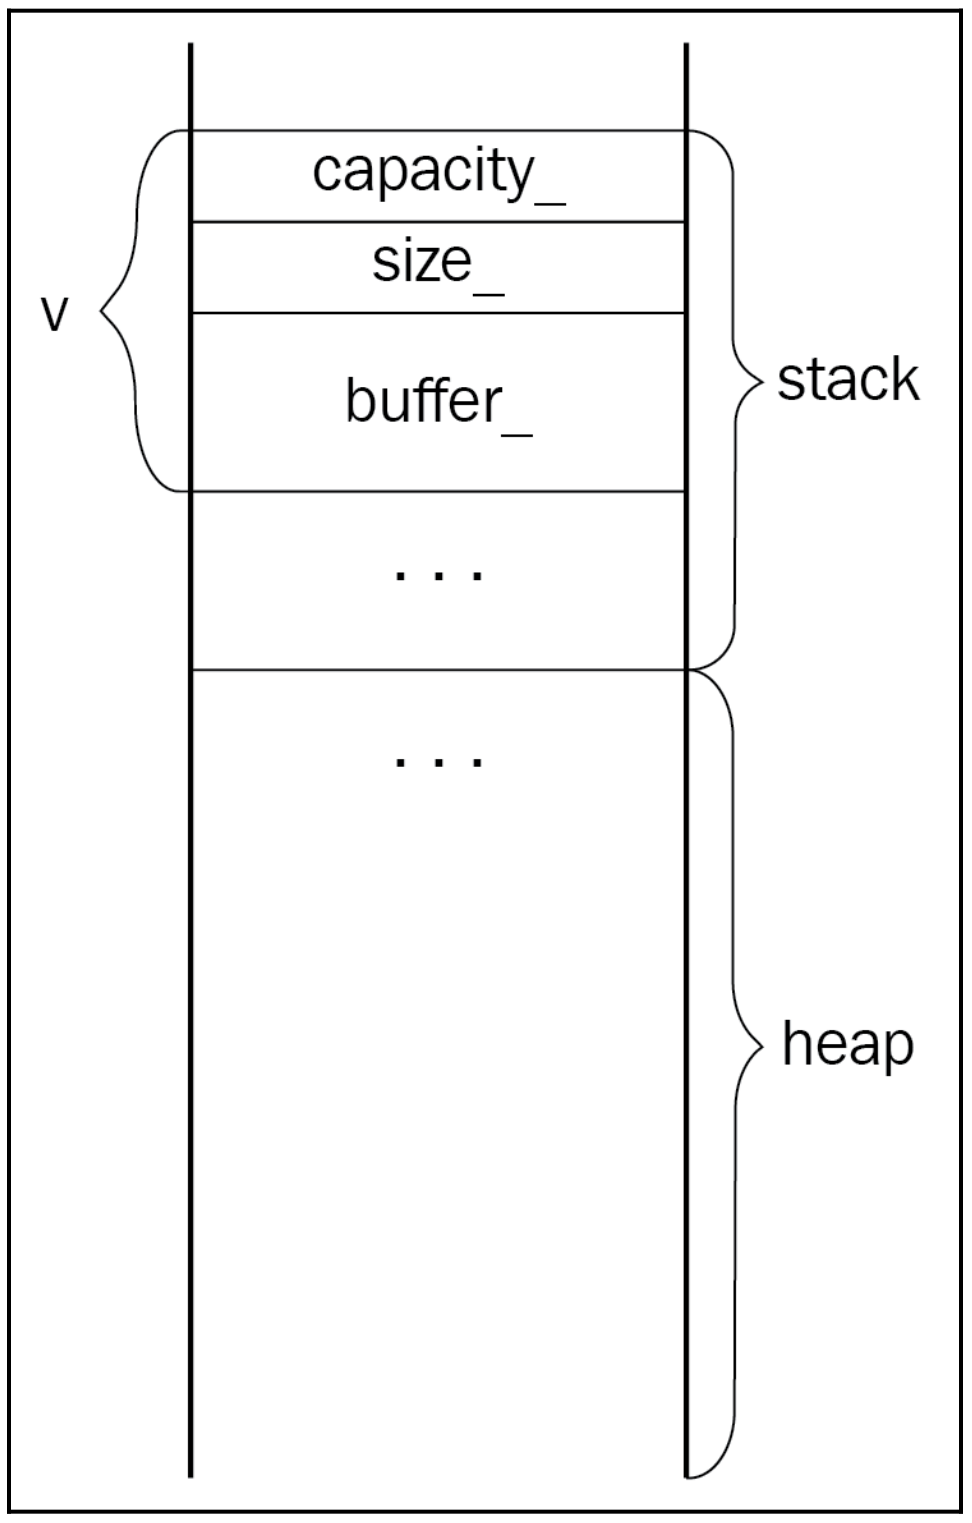
\includegraphics[width=0.4\textwidth]{content/Section-2/Chapter-6/9}
\end{center}

插入元素之后,堆栈上的vector对象的大小将保持不变,堆来保存现场。buffer\underline{ }数组指向一个使用new[]操作符分配的内存位置。例如下面的代码: \par

\begin{lstlisting}[caption={}]
// we continue the code from previous listing
v.push_back(17);
v.push_back(21);
v.push_back(74);
\end{lstlisting}

每一个推入vector的新元素都将占用堆中的空间,如下图所示: \par

\begin{center}
	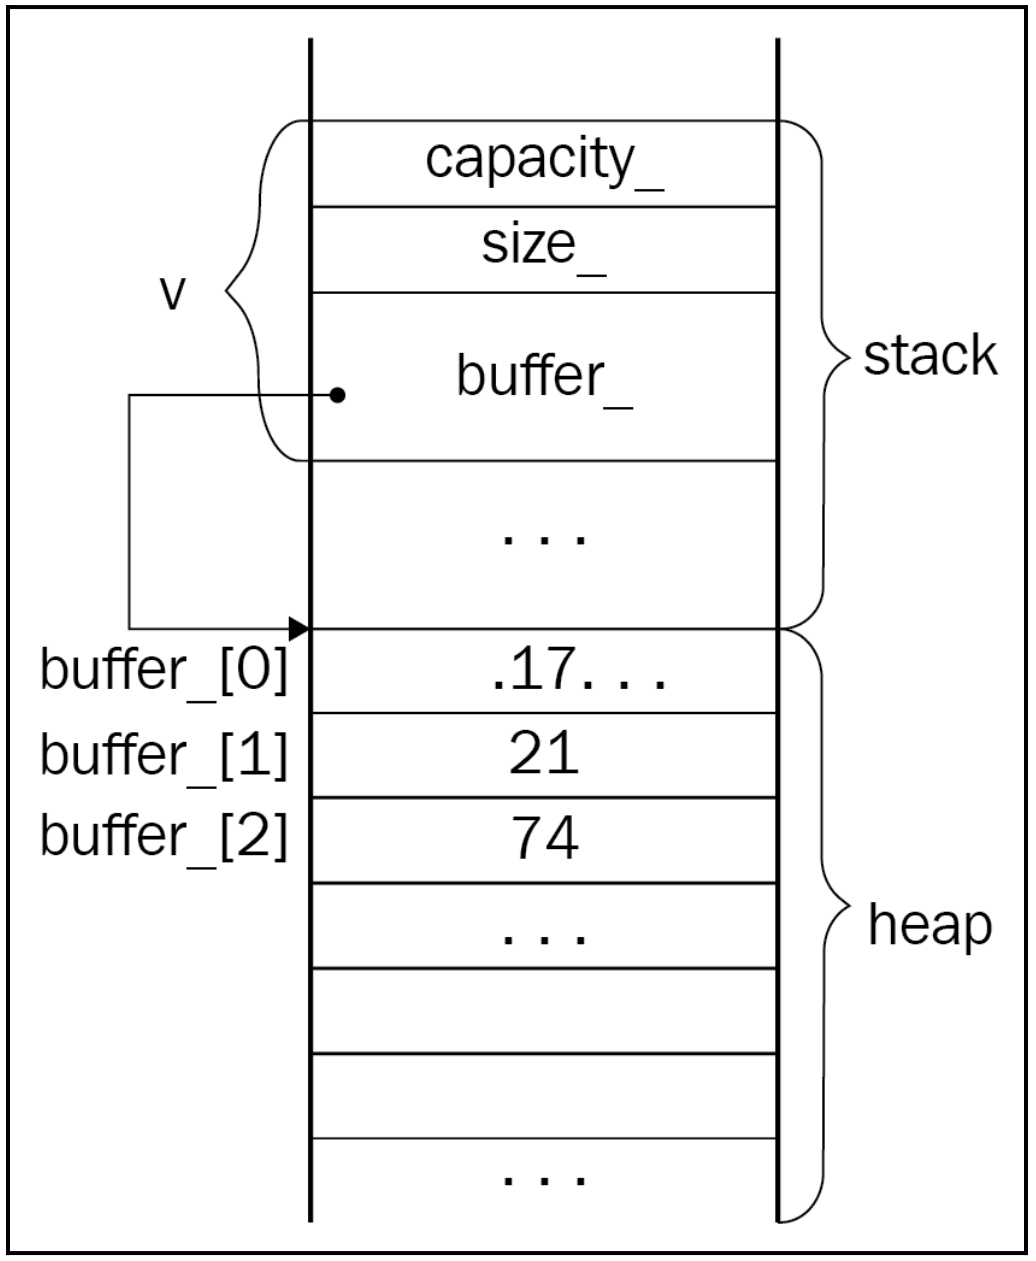
\includegraphics[width=0.6\textwidth]{content/Section-2/Chapter-6/10}
\end{center}

每个新插入的元素都位于buffer\underline{ }数组的最后。这就是为什么我们可以说vector是一个对缓存友好的容器。 \par
声明一个链表对象也会在堆栈上,为其数据成员占用内存空间。如果讨论只存储head\underline{ }指针的简单实现,那么下面的list对象声明将占用至少8个字节的内存(仅针对head\underline{ }指针): \par

\begin{lstlisting}[caption={}]
int main()
{
	LinkedList<int> list;
}
\end{lstlisting}

下面的图描述了上述代码的内存布局: \par

\begin{center}
	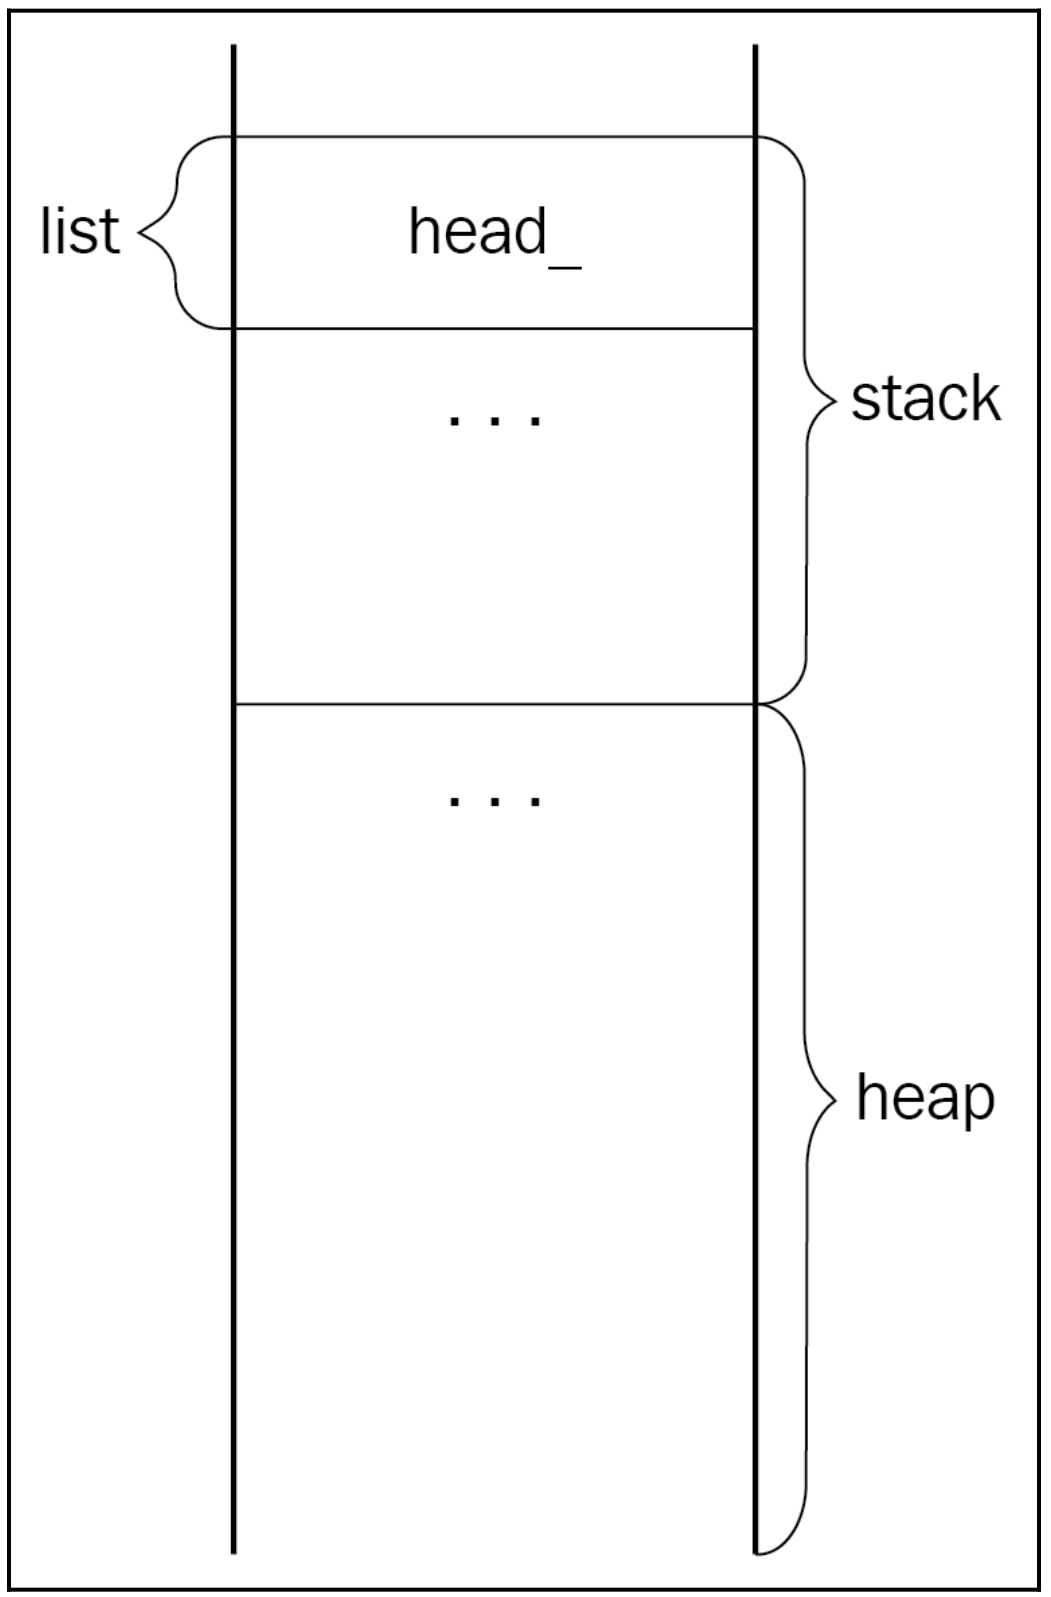
\includegraphics[width=0.4\textwidth]{content/Section-2/Chapter-6/11}
\end{center}

插入新元素会在堆上创建一个node类型的对象。看看下面这行: \par

\begin{lstlisting}[caption={}]
list.push_back(19);
\end{lstlisting}

下面是插入新元素后内存图的变化: \par

\begin{center}
	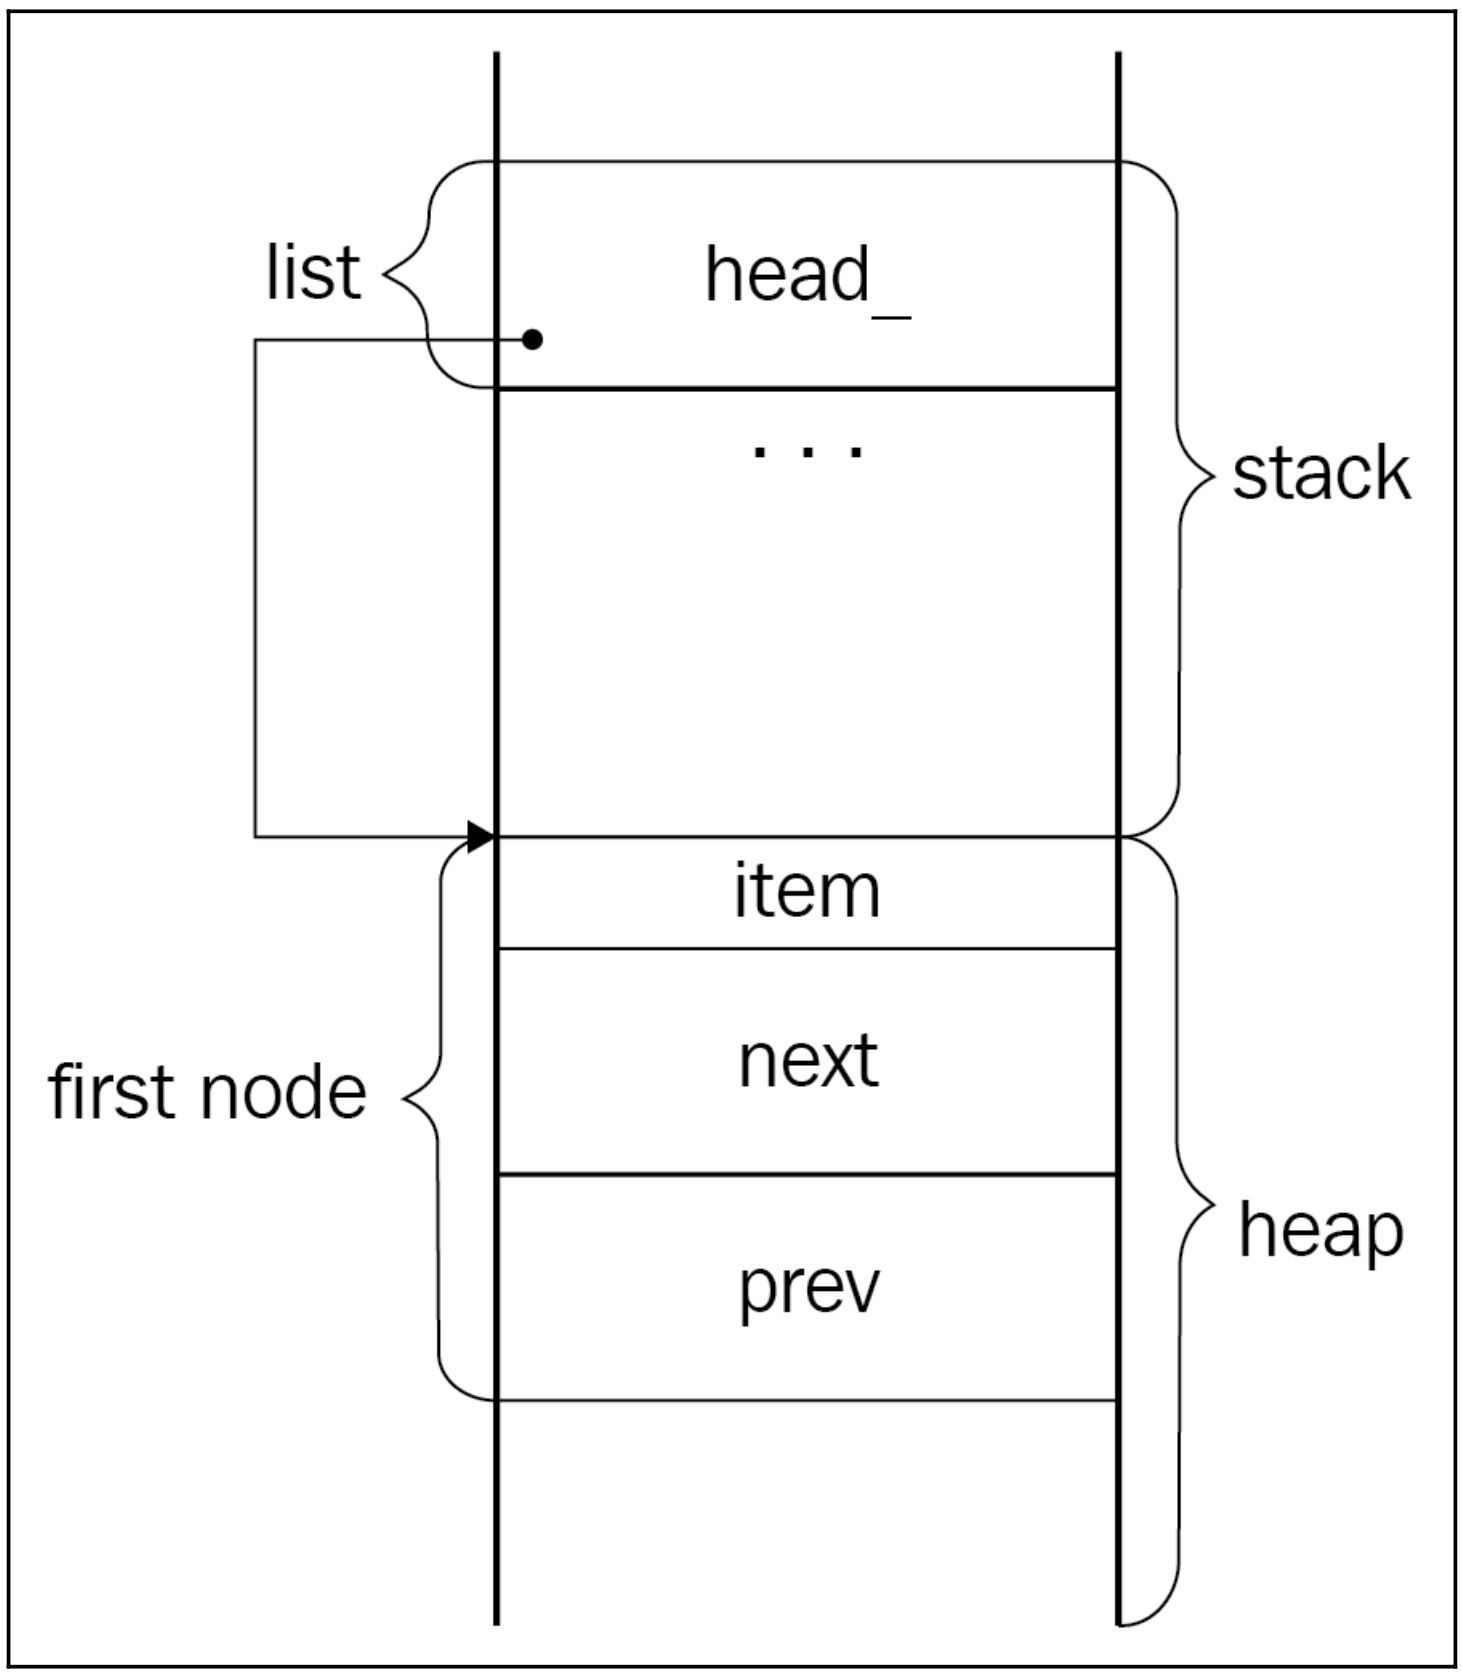
\includegraphics[width=0.6\textwidth]{content/Section-2/Chapter-6/12}
\end{center}

注意,节点的所有数据成员都驻留在堆上,item存储我们要插入的值。当我们插入另一个元素时,将再次创建一个新节点。这次,第一个节点的下一个指针将指向新插入的元素。新插入节点的prev指针将指向列表的前一个节点。下图描述了插入第二个元素后链表的内存布局: \par

\begin{center}
	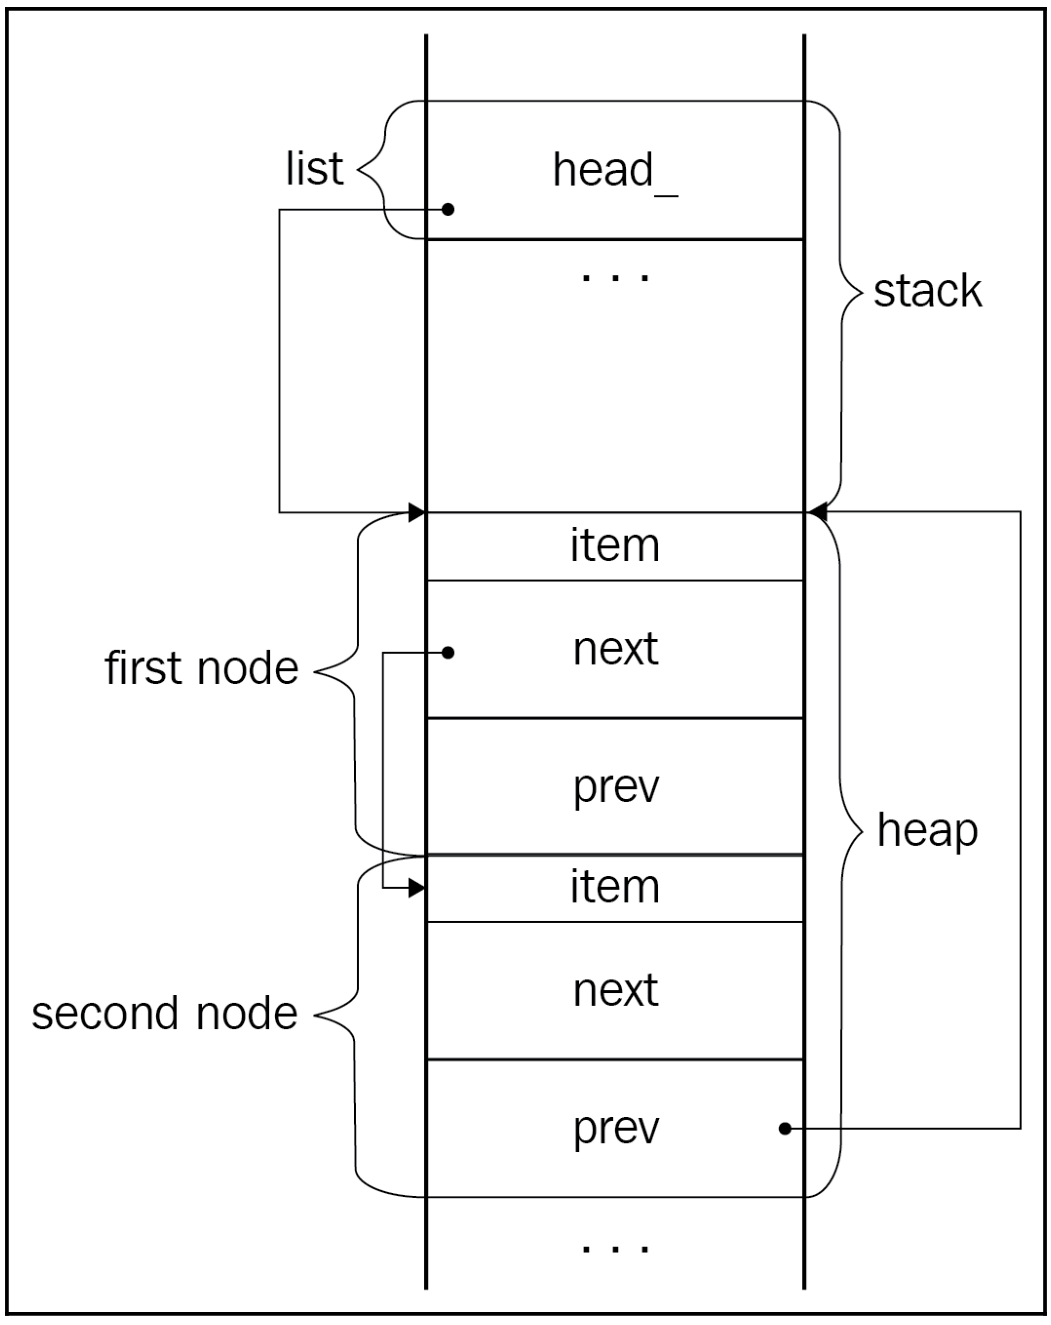
\includegraphics[width=0.6\textwidth]{content/Section-2/Chapter-6/13}
\end{center}

当向列表中插入元素的过程中在堆上分配一些随机对象时,会发生有趣的事情。例如,下面的代码将一个节点插入到列表中,然后为一个整数(与列表无关)分配空间。最后,再次向列表中插入一个元素: \par

\begin{lstlisting}[caption={}]
int main()
{
	LinkedList<int> list;
	list.push_back(19);
	int* random = new int(129);
	list.push_back(22);
}
\end{lstlisting}

这种中间随机对象声明破坏了列表元素的顺序,如下图所示: \par

\begin{center}
	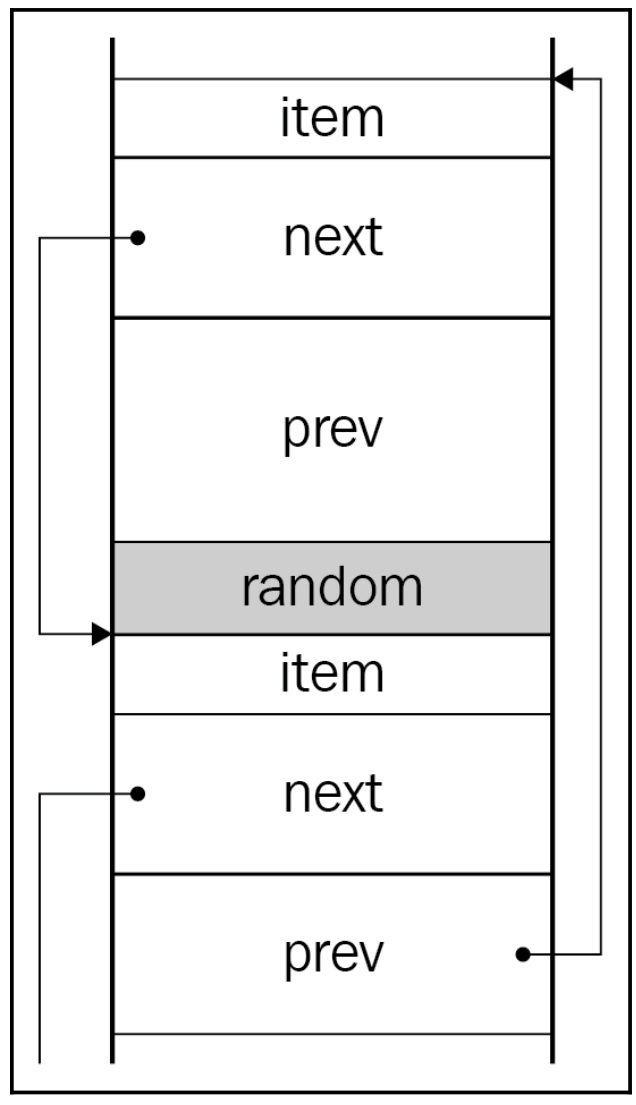
\includegraphics[width=0.4\textwidth]{content/Section-2/Chapter-6/14}
\end{center}

上面的图提示我们,由于列表的结构和元素的分配,它不是一个缓存友好的容器。 \par

\hspace*{\fill} \\ %插入空行

\includegraphics[width=0.05\textwidth]{images/tip}
请注意将每个新节点合并到代码中所产生的内存开销,我们为一个元素额外使用了16个字节(考虑到指针需要8个字节的内存)。因此,在最佳内存使用的比拼中,列表输给了vector。 \par
\noindent\textbf{}\ \par

我们可以通过在列表中引入一个预先分配的缓冲区来解决这个问题。然后,每个新节点的创建都将通过重新实现的new操作符传递。更明智的做法是选择更适合问题的数据结构。 \par
实际的应用程序开发中,开发者很少自己实现向量或链表,通常会使用经过测试的稳定库版本。C++同时提供了vector和链表的标准容器。此外,为单链表和双链表提供了独立的两个容器。 \par

\noindent\textbf{}\ \par
\textbf{STL容器} \ \par
STL是一个强大的算法和容器集合。虽然理解和实现数据结构对程序员来说是一项很好的技能,但不必在项目中每次都去实现它们。标准库库提供商负责为我们实现稳定的、经过测试的数据结构和算法。通过了解数据结构和算法的细节,在解决问题时更好地选择STL容器和算法。 \par
前面讨论的vector和链表在STL中实现为std::vector<T>和std::list<T>,其中T是容器中每个元素的类型。除了类型之外,容器还接受分配器作为第二个默认模板参数。例如,std::vector的声明如下: \par

\begin{lstlisting}[caption={}]
template <typename T, typename Allocator = std::allocator<T> >
class vector;
\end{lstlisting}

正如前一章所介绍的,分配器处理容器元素的分配/回收。std::allocator是STL中所有标准容器的默认分配器。一个更复杂的基于内存资源行为不同的分配器是std::pmr::polymorphic\underline{ }allocator。STL提供了std::pmr::vector作为使用多态分配器的别名模板,定义如下: \par

\begin{lstlisting}[caption={}]
namespace pmr {
	template <typename T>
	using vector = std::vector<T, std::pmr::polymorphic_allocator<T>>;
}
\end{lstlisting}

现在让我们来仔细的了解下std::vector和std::list。  \par

\noindent\textbf{}\ \par
\textbf{使用std::vector和std::list} \ \par
std::vector定义在<vector>头文件中。最简单的用法示例: \par

\begin{lstlisting}[caption={}]
#include <vector>

int main()
{
	std::vector<int> vec;
	vec.push_back(4);
	vec.push_back(2);
	for (const auto& elem : vec) {
		std::cout << elem;
	}
}
\end{lstlisting}

vector是动态增长的,应该考虑增长因素。声明vector时,有默认的容量,然后在插入元素时增长。每当元素的数量超过vector的容量时,vector就将容量增加一个给定的因子(通常是将容量翻倍)的量。如果我们知道vector中需要的元素的大致数量,可以通过使用reserve()方法首先为vector分配容量来优化它的使用。例如,下面的代码保留了10,000个元素的容量: \par

\begin{lstlisting}[caption={}]
std::vector<int> vec;
vec.reserve(10000);
\end{lstlisting}

它强制vector为10,000个元素分配空间,从而避免在元素插入期间调整大小(除非达到10,000个元素的阈值)。 \par
另一方面,如果遇到容量远远大于vector中实际元素数量的情况,则可以收缩vector以释放未使用的内存。我们需要调用shrink\underline{ }to\underline{ }fit()函数,如下面的示例所示: \par

\begin{lstlisting}[caption={}]
vec.shrink_to_fit();
\end{lstlisting}

访问vector元素的方法与访问普通数组的方法相同,使用操作符[]。但是,std::vector提供了两个访问其元素的选项。其中一种方法认为是安全的,通过at()函数完成,如下所示: \par

\begin{lstlisting}[caption={}]
std::cout << vec.at(2);
// is the same as
std::cout << vec[2];
// which is the same as
std::cout << vec.data()[2];
\end{lstlisting}

at()和操作符[]的区别在于,at()访问指定元素时进行边界检查,下面一行抛出了一个std::out\underline{ }of\underline{ }range异常: \par

\begin{lstlisting}[caption={}]
try {
	vec.at(999999);
} catch (std::out_of_range& e) { }
\end{lstlisting}

我们几乎以同样的方式使用std::list。这些列表大多具有类似的公共接口。本章后面,我们将讨论允许从特定容器中抽象的迭代器,这样就可以用vector替换list,而不会有太多损失。在此之前,让我们看看list和vector的公共接口的区别。 \par
除了这两个容器都支持的标准函数集,如size()、resize()、empty()、clear()、erase()等,列表还有push\underline{ }front()函数,用于在列表的前插入一个元素。因为std::list表示一个双向链表。如下代码所示,std::list也支持push\underline{ }back(): \par

\begin{lstlisting}[caption={}]
std::list<double> lst;
lst.push_back(4.2);
lst.push_front(3.14);
// the list contains: "3.14 -> 4.2"
\end{lstlisting}

列表的添加操作,在许多情况下会派上用场。例如,要合并两个排序列表,我们使用merge()方法。它接受另一个列表作为参数,并将其所有元素移动到当前列表中。作为参数传递给merge()方法的列表在操作之后变为空。 \par

\hspace*{\fill} \\ %插入空行

\includegraphics[width=0.05\textwidth]{images/tip}
STL还提供了一个单链表,用std::forward\underline{ }list表示。要使用它,你应该包含<forward\underline{ }list>头文件。由于单链表节点只有一个指针,因此它比双链表更省内存。 \par
\noindent\textbf{}\ \par

splice()方法类似于merge(),不同的是它移动作为参数提供的一部分,通过移动将内部指针重新指向合适的列表节点。merge()和splice()都是如此。 \par
当我们使用容器存储和操作复杂对象时,复制元素的代价在程序的性能中扮演着重要的角色。考虑下面一个三维点的结构体: \par

\begin{lstlisting}[caption={}]
struct Point
{
	float x;
	float y;
	float z;
	Point(float px, float py, float pz)
	: x(px), y(py), z(pz)
	{}
	Point(Point&& p)
	: x(p.x), y(p.y), z(p.z)
	{}
};
\end{lstlisting}

现在,将一个Point对象插入到vector中: \par

\begin{lstlisting}[caption={}]
std::vector<Point> points;
points.push_back(Point(1.1, 2.2, 3.3));
\end{lstlisting}

构造一个临时对象,然后移动到向量对应的槽中。我们可以直观地表示为: \par

\begin{center}
	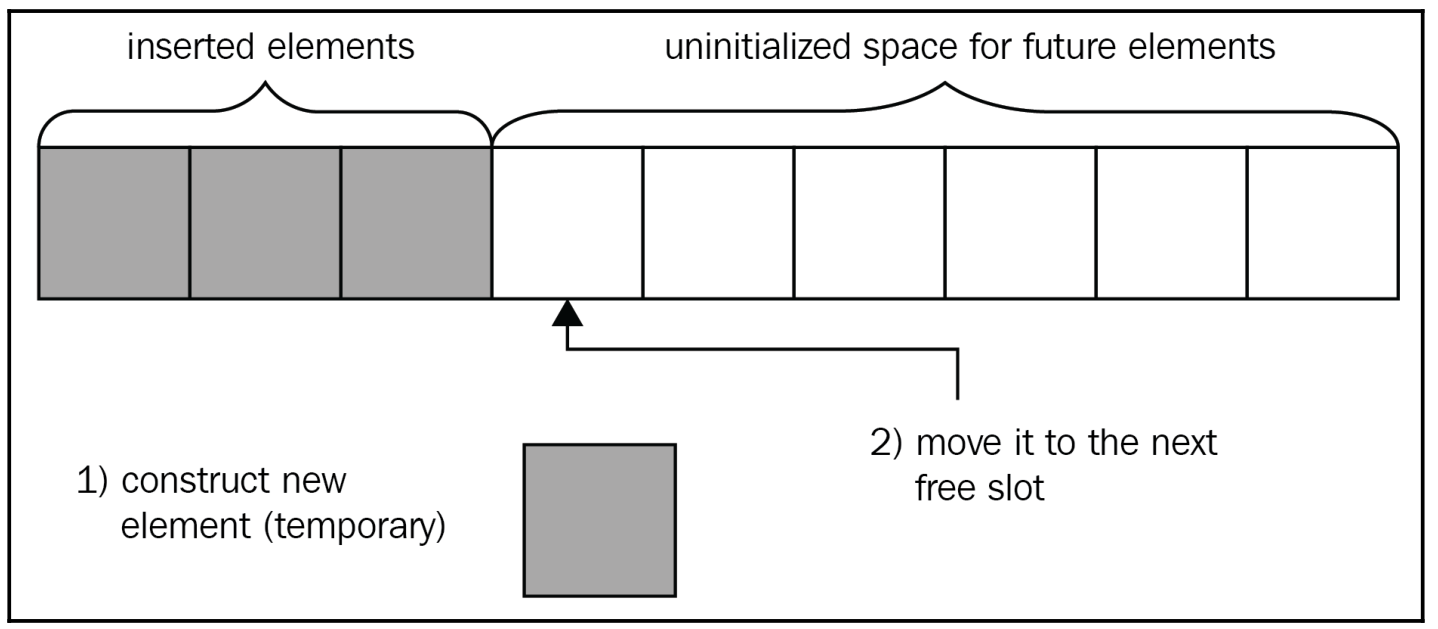
\includegraphics[width=0.6\textwidth]{content/Section-2/Chapter-6/15}
\end{center}

vector会提前占用更多的空间,从而尽可能长地延迟调整操作。当插入新元素时,vector会将其复制到下一个可用的槽位(如果槽位已满,则会重新分配更多空间)。我们可以使用未初始化的空间在适当位置创建新元素。为此,vector提供了emplace\underline{ }back()函数。 \par

\begin{lstlisting}[caption={}]
points.emplace_back(1.1, 2.2, 3.3);
\end{lstlisting}

请注意这里直接传递给函数的参数。下图描述了emplace\underline{ }back()的用法: \par

\begin{center}
	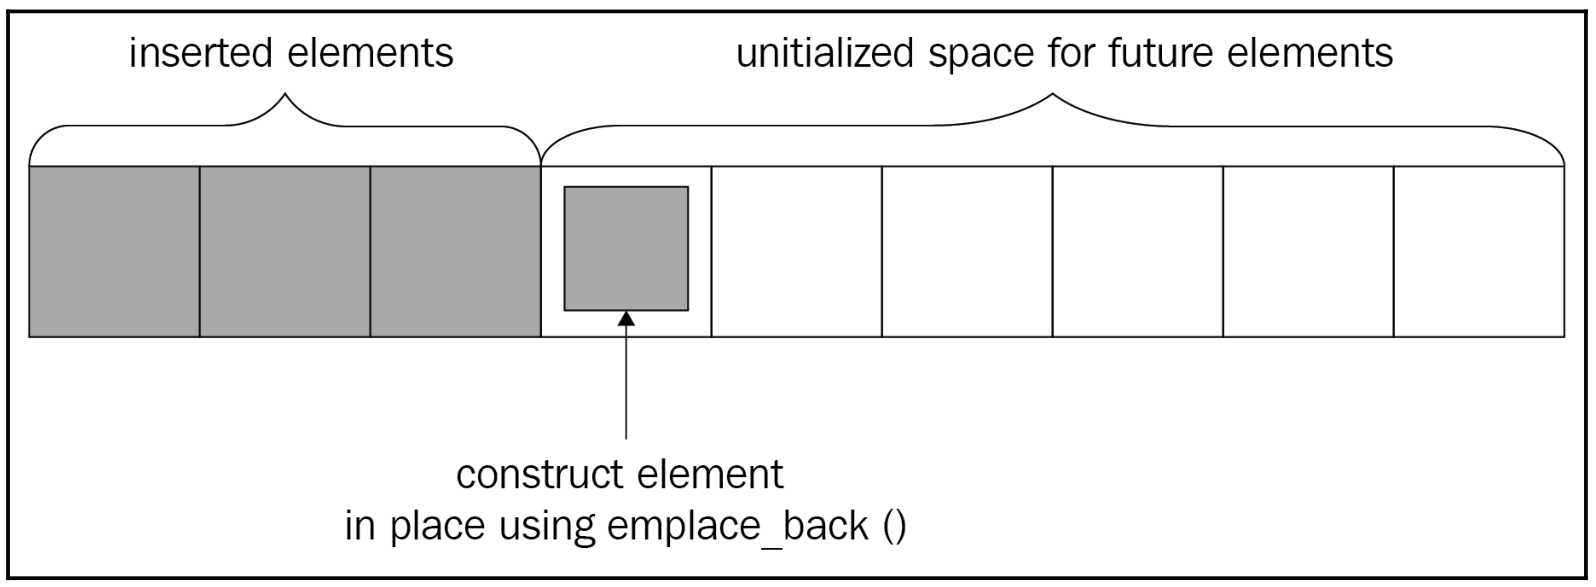
\includegraphics[width=0.6\textwidth]{content/Section-2/Chapter-6/16}
\end{center}

emplace\underline{ }back()通过std::allocator\underline{ }traits::construct()构造元素。后者通常使用new操作符在已经分配的未初始化空间中构造元素。 \par
std::list还提供了一个emplace\underline{ }front()方法。这两个函数都返回对插入元素的引用。唯一的要求是元素的类型必须是EmplaceConstructible。对于vector,类型也应该是MoveInsertable。 \par

\noindent\textbf{}\ \par
\textbf{使用容器适配器} \ \par
作为开发者可能遇到过将堆栈和队列描述为数据结构(或者用C++来表示容器)的情况。从技术上讲,它们不是数据结构,而是数据结构适配器。STL中,std::stack和std::queue通过提供访问容器的特殊接口来适配容器。堆栈这个词几乎无处不在,到目前为止,我们已经使用它来描述具有自动存储时间对象的内存段。由于分配/回收策略,这段内存称为堆栈。 \par
我们说对象在每次声明时都会入栈,在销毁时出栈。对象的弹出顺序与它们推入顺序相反。这就是将内存段调用堆栈的原因,同样的后进先出(LIFO)方法也适用于堆栈适配器。std::stack提供的关键功能如下: \par

\begin{lstlisting}[caption={}]
void push(const value_type& value);
void push(value_type&& value);
\end{lstlisting}

push()函数有效地调用了底层容器的push\underline{ }back()。通常,堆栈是使用vector来实现的。在介绍保护继承时,已经在第3章中讨论过这样的场景。stack有两个模板形参,其中一个是容器。选择什么并不重要,但它必须有push\underline{ }back()成员函数。std::stack和std::queue的默认容器是std::deque。\par
std::deque允许在开头和结尾快速插入,是一个类似于std::vector的索引顺序容器。名称deque表示双端队列。 \par
让我们看看堆栈的行为: \par

\begin{lstlisting}[caption={}]
#include <stack>

int main()
{
	std::stack<int> st;
	st.push(1); // stack contains: 1
	st.push(2); // stack contains: 2 1
	st.push(3); // stack contains: 3 2 1
}
\end{lstlisting}

替代push()函数更好的方法是emplace()。因此,调用底层容器的emplace\underline{ }back(),在适当的位置构造元素。 \par
为了取出元素,我们调用pop()函数。它不接受任何参数,也不返回任何东西,它只是从堆栈中删除顶部元素。要访问堆栈的顶部元素,需要调用top()函数。修改前面的例子,在弹出堆栈元素之前打印所有的堆栈元素: \par

\begin{lstlisting}[caption={}]
#include <stack>
int main()
{
	std::stack<int> st;
	st.push(1);
	st.push(2);
	st.push(3);
	std::cout << st.top(); // prints 3
	st.pop();
	std::cout << st.top(); // prints 2
	st.pop();
	std::cout << st.top(); // prints 1
	st.pop();
	std::cout << st.top(); // crashes application
}
\end{lstlisting}

函数的作用:返回对顶部元素的引用,调用底层容器的back()函数。请注意在空堆栈上调用的最后一个top()函数。我们建议在对空堆栈调用top()之前,使用size()检查堆栈的大小。 \par
queue是另一个适配器,与栈的行为略有不同。队列背后的逻辑是,它首先返回第一个插入的元素:先进先出(FIFO)原则。 \par

\begin{center}
	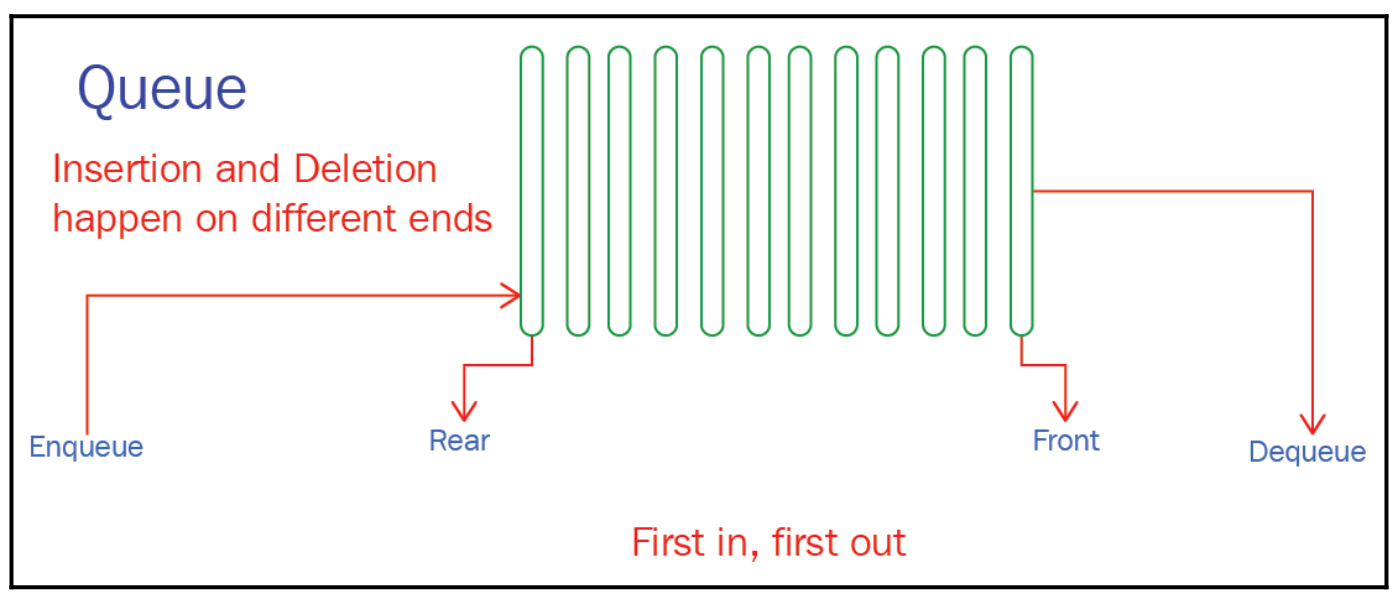
\includegraphics[width=0.6\textwidth]{content/Section-2/Chapter-6/17}
\end{center}

队列中插入和检索操作的正式名称是enqueue和dequeue。queue保持数据一致性的方法,并提供push()和pop()函数。要访问队列的第一个和最后一个元素,应该使用front()和back(),两者都返回对元素的引用。下面是一个简单的用法示例: \par

\begin{lstlisting}[caption={}]
#include <queue>
int main()
{
	std::queue<char> q;
	q.push('a');
	q.push('b');
	q.push('c');
	std::cout << q.front(); // prints 'a'
	std::cout << q.back(); // prints 'c'
	q.pop();
	std::cout << q.front(); // prints 'b'
}
\end{lstlisting}

要正确使用各种容器和适配器时,了解它们是很有必要的。在为各种问题选择合适的容器方面,并没有什么灵丹妙药。许多编译器使用堆栈来解析代码表达式,例如:很容易使用栈,验证下面表达式中的圆括号: \par

\begin{lstlisting}[caption={}]
int r = (a + b) + (((x * y) - (a / b)) / 4);
\end{lstlisting}

试着练习一下。编写一个小程序,使用堆栈验证前面的表达式。 \par
另一个容器适配器是std::priority\underline{ }queue。优先队列通常采用均衡的、基于节点的数据结构,比如:大堆或小堆。我们将在本章的末尾研究树和图,以及了解优先队列是如何工作的。 \par

\noindent\textbf{}\ \par
\textbf{迭代容器} \ \par
不可迭代的容器就像不能驾驶的汽车。毕竟,容器是项的集合,循环遍历容器元素的一种常用方法是使用普通的for循环: \par

\begin{lstlisting}[caption={}]
std::vector<int> vec{1, 2, 3, 4, 5};
for (int ix = 0; ix < vec.size(); ++ix) {
	std::cout << vec[ix];
}
\end{lstlisting}

容器为元素访问提供了一组不同的操作。例如,vector提供操作符[],而list没有。std::list有front()和back()方法,它们分别返回第一个和最后一个元素。如前所述,std::vector还提供了at()和运算符[]。 \par
这意味着不能使用前面的循环来迭代列表元素。但可以使用基于范围的for循环遍历列表(和vector),如下所示: \par

\begin{lstlisting}[caption={}]
std::list<double> lst{1.1, 2.2, 3.3, 4.2};
for (auto& elem : lst) {
	std::cout << elem;
}
\end{lstlisting}

看起来可能令人困惑,这个技巧隐藏在基于范围的实现中。它使用std::begin()函数检索指向容器第一个元素的迭代器。 \par 
迭代器是指向容器元素的对象,可以根据容器的物理结构推进到下一个元素。下面的代码声明了一个vector迭代器,并使用指向vector开头的迭代器对其进行初始化: \par

\begin{lstlisting}[caption={}]
std::vector<int> vec{1, 2, 3, 4};
std::vector<int>::iterator it{vec.begin()};
\end{lstlisting}

容器提供了两个成员函数begin()和end(),分别返回指向容器开头和结尾的迭代器。下面的图表显示了如何处理容器的开头和结尾: \par

\begin{center}
	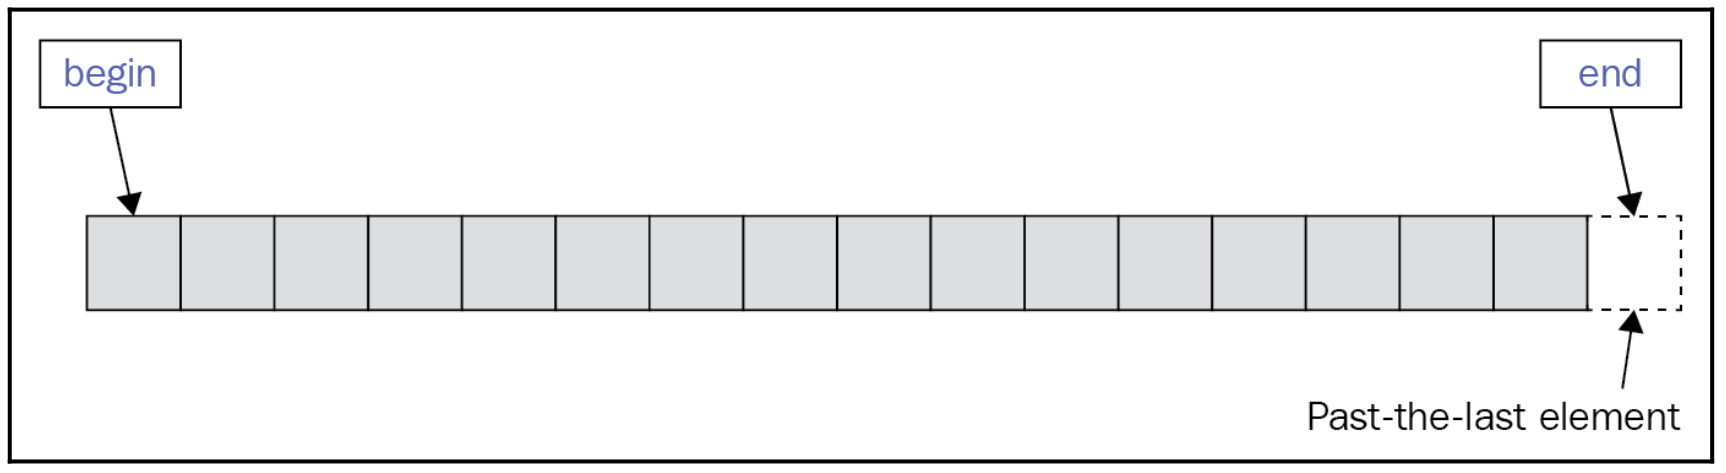
\includegraphics[width=0.6\textwidth]{content/Section-2/Chapter-6/18}
\end{center}

前面使用基于范围的for遍历列表元素的代码,可以认为类似于以下代码: \par

\begin{lstlisting}[caption={}]
auto it_begin = std::begin(lst);
auto it_end = std::end(lst);
for ( ; it_begin != it_end; ++it_begin) {
	std::cout << *it_begin;
}
\end{lstlisting}

请注意前面代码中使用的*操作符,该操作符通过迭代器访问底层元素。我们认为迭代器是指向容器元素的指针。 \par

\hspace*{\fill} \\ %插入空行

\includegraphics[width=0.05\textwidth]{images/tip}
std::begin()和std::end()函数通常分别调用容器的begin()和end()方法,也适用于常规数组。 \par
\noindent\textbf{}\ \par

容器迭代器清楚地知道如何使用容器元素,例如:向前移动vector迭代器将其移动到数组的下一个槽位,而向前移动list迭代器则使用相应的指针将其移动到下一个节点,如下面的代码所示: \par

\begin{lstlisting}[caption={}]
std::vector<int> vec;
vec.push_back(4);
vec.push_back(2);
std::vector<int>::iterator it = vec.begin();
std::cout << *it; // 4
it++;
std::cout << *it; // 2

std::list<int> lst;
lst.push_back(4);
lst.push_back(2);
std::list<int>::iterator lit = lst.begin();
std::cout << *lit; // 4
lit++;
std::cout << *lit; // 2
\end{lstlisting}

每个容器都有自己的迭代器实现,这就是为什么list迭代器和vector迭代器有相同的接口,但行为不同。迭代器的行为由它的类别定义,例如:vector的迭代器是随机访问迭代器,可以使用该迭代器随机访问任何元素。下面的代码通过vector的迭代器向vector的第4个元素添加3,如下所示: \par

\begin{lstlisting}[caption={}]
auto it = vec.begin();
std::cout << *(it + 3);
\end{lstlisting}

STL中有六种类型的迭代器: \par

\begin{itemize}
	\item 输入
	\item 输出(与输入相同,但支持写访问)
	\item 向前
	\item 双向
	\item 随机访问
	\item 连续性
\end{itemize}

输入迭代器提供读访问(通过调用*操作符),并允许使用前缀和后缀自增操作符转发迭代器位置。输入迭代器不支持多次传递,只能使用迭代器在容器上迭代一次。另一方面,前向迭代器支持多次传递,支持多次遍历可以通过迭代器多次读取元素的值。 \par
输出迭代器不提供对元素的访问,但它允许给元素赋新值。具有多重传递特性的输入迭代器和输出迭代器的组合构成了前向迭代器。然而,前向迭代器只支持自增操作,而双向迭代器支持将迭代器移动到任何位置。它们都支持递减操作,例如:std::list支持双向迭代器。 \par
最后,随机访问迭代器允许通过在迭代器上加/减一个数字来跳转元素。迭代器将跳转到算术操作指定的位置。vector提供了随机访问迭代器。 \par
每个类别都定义了一组可应用于迭代器的操作,例如:可以使用输入迭代器读取元素的值,并通过递增迭代器前进到下一个元素。另一方面,随机访问迭代器允许迭代器对任意值递增或递减,读取和写入元素的值等。 \par
本节描述的所有特性的组合都属于连续迭代器类别,它也期望容器是连续的。这意味着容器元素需要紧挨着另一个元素。连续容器的经典例子是std::array。 \par
像distance()这样的函数使用迭代器的信息来实现最快的执行结果。例如,两个双向迭代器之间的distance()函数的执行时间是线性的,而用于随机访问迭代器相同函数的执行时间是常量。 \par
下面的伪代码演示了一个示例实现: \par

\begin{lstlisting}[caption={}]
template <typename Iter>
std::size_type distance(Iter first, Iter second) {
	if (Iter is a random_access_iterator) {
		return second - first;
	}
	std::size_type count = 0;
	for ( ; first != last; ++count, first++) {}
	return count;
}
\end{lstlisting}

尽管前面示例中显示的伪代码工作良好,但我们应该考虑在运行时检查迭代器的类别不是一个选项。它是在编译时定义的,因此需要使用模板特化来为随机访问迭代器生成distance()函数。更好的解决方案是使用std::is\underline{ }same类型特征,定义在<type\underline{ }traits>中: \par

\begin{lstlisting}[caption={}]
#include <iterator>
#include <type_traits>

template <typename Iter>
typename std::iterator_traits<Iter>::difference_type distance(Iter first,
Iter last)
{
	using category = std::iterator_traits<Iter>::iterator_category;
	if constexpr (std::is_same_v<category, std::random_access_iterator_tag>)
	{
		return last - first;
	}
	typename std::iterator_traits<Iter>::difference_type count;
	for (; first != last; ++count, first++) {}
	return count;
}
\end{lstlisting}

std::is\underline{ }same\underline{ }v是std::is\underline{ }same的助手模板,定义如下: \par

\begin{lstlisting}[caption={}]
template <class T, class U>
inline constexpr bool is_same_v = is_same<T, U>::value;
\end{lstlisting}

迭代器最重要的特性是,减少了容器和算法之间的耦合: \par

\begin{center}
	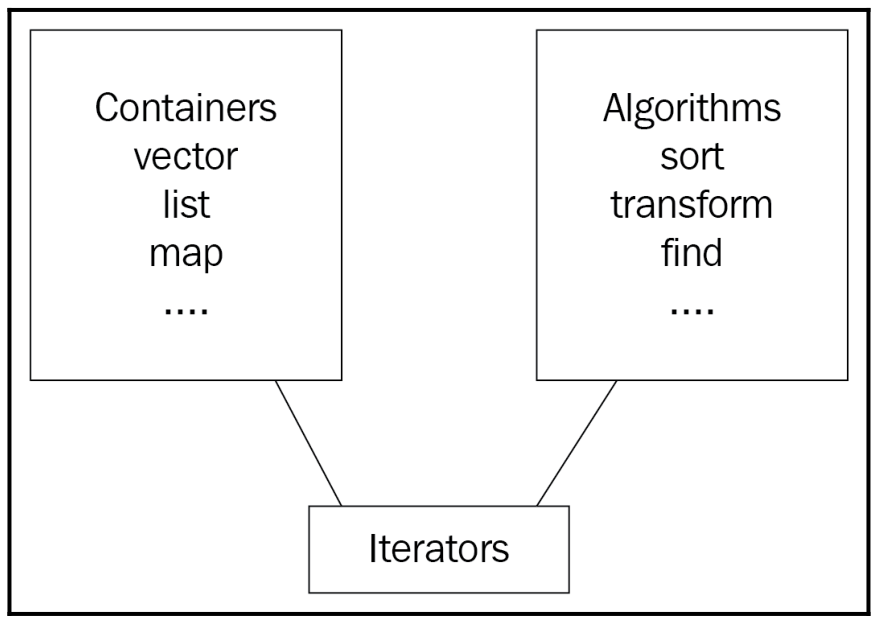
\includegraphics[width=0.4\textwidth]{content/Section-2/Chapter-6/19}
\end{center}

STL基于这三个概念:容器、算法和迭代器。虽然vector、list或任何其他容器不同,但它们都有相同的目的:存储数据。 \par
另一方面,算法是处理数据的函数,大部分时间都在收集数据。算法定义通常表示一种通用的方式,指定应该采取的步骤来处理容器元素。例如,排序算法按升序或降序对容器元素进行排序。 \par
vector是连续容器,而list是基于节点的容器。对它们进行排序需要对特定容器的物理结构有更深入的了解。要正确地对向量进行排序,应该为它实现一个单独的排序函数。 \par
迭代器将这种实现的多样性带到通用级别。它们为库设计人员提供了实现一个排序函数的能力,该函数将只处理迭代器,从容器类型中抽象出来。STL中使用sort()算法(在<algorithm>中定义)处理迭代器,我们可以用同一个函数对向量和列表进行排序: \par

\begin{lstlisting}[caption={}]
#include <algorithm>
#include <vector>
#include <list>
...
std::vector<int> vec;
// insert elements into the vector
std::list<int> lst;
// insert elements into the list

std::sort(vec.begin(), vec.end());
std::sort(lst.begin(), lst.end());
\end{lstlisting}

本节中描述的迭代器现在认为是之前版本遗留特性,C++20引入了一种新的基于概念的迭代器。 \par

\noindent\textbf{}\ \par
\textbf{概念和迭代器} \ \par
C++20的主要特性之一是引入概念。除了概念之外,C++20还提供了基于概念的新迭代器。虽然本章讨论的迭代器现在认为是遗留特性,但已经用它们编写了许多代码。这就是我们在继续讨论新的迭代器概念之前.首先介绍它们的原因。现在,让我们来看看,什么是概念,以及如何使用。 \par

\noindent\textbf{}\ \par
\textbf{理解概念} \ \par
抽象在计算机编程中是必不可少,在第3章介绍了类,作为一种将数据和操作表示为抽象实体的方法。在第4章中,我们深入探讨了模板,并了解了如何通过对各种聚合类型重用模板,从而使类变得更加灵活。模板不仅提供特定类型的抽象,还可以去除实体类型和聚合类型之间的耦合。以std::vector为例,它提供了通用接口来存储和操作对象集合。我们声明三个不同的vector,包含三种不同类型的对象,如下所示: \par

\begin{lstlisting}[caption={}]
std::vector<int> ivec;
std::vector<Person> persons;
std::vector<std::vector<double>> float_matrix;
\end{lstlisting}

如果不是模板,我们必须对前面的代码做如下操作: \par

\begin{lstlisting}[caption={}]
std::int_vector ivec;
std::custom_vector persons; // supposing the custom_vector stores void*
std::double_vector_vector float_matrix;
\end{lstlisting}

尽管这段的代码无法可接受,但应该认可模板是泛型编程的基础这一事实。概念为泛型编程引入了更多的灵活性。现在可以对模板参数设置限制,检查约束,并在编译时发现不一致的行为。模板类声明如下: \par

\begin{lstlisting}[caption={}]
template <typename T>
class Wallet
{
	// the body of the class using the T type
};
\end{lstlisting}

请注意前面代码块中的typename关键字。概念允许用描述模板形参的类型,来替换模板形参。假设我们想让Wallet使用可以添加的类型,应该是可添加的。下面是如何使用概念来帮助代码实现的: \par

\begin{lstlisting}[caption={}]
template <addable T>
class Wallet
{
	// the body of the class using addable T's
};
\end{lstlisting}

现在可以通过可添加的类型来创建Wallet的实例。当类型不满足约束时,编译器将抛出错误。下面的代码片段声明了两个Wallet对象: \par

\begin{lstlisting}[caption={}]
class Book
{
	// doesn't have an operator+
	// the body is omitted for brevity
};
constexpr bool operator+(const Money& a, const Money& b) {
	return Money{a.value_ + b.value_};
}

class Money
{
	friend constexpr bool operator+(const Money&, const Money&);
	// code omitted for brevity
private:
	double value_;
}; 

Wallet<Money> w; // works fine
Wallet<Book> g; // compile error
\end{lstlisting}

Book类没有加法操作符,因此由于模板形参类型的限制,g的构造将失败。 \par
概念的声明是使用concept关键字完成的,其形式如下: \par

\begin{lstlisting}[caption={}]
template <parameter-list>
concept name-of-the-concept = constraint-expression;
\end{lstlisting}

概念也使用模板声明,我们可以将它们称为描述类型的类型。概念在很大程度上依赖于约束。约束是为模板参数指定要求的一种方式,而概念是一组约束。下面是我们如何实现前面的可添加概念: \par

\begin{lstlisting}[caption={}]
template <typename T>
concept addable = requires (T obj) { obj + obj; }
\end{lstlisting}

标准概念定义在<concepts>头文件中。 \par
我们还可以通过要求新概念支持其他概念来将几个概念组合成一个概念。使用\&\&操作符,让看看迭代器是如何利用概念的,并举例说明结合了其他概念的可递增迭代器概念。 \par

\noindent\textbf{}\ \par
\textbf{C++20中使用迭代器} \ \par
介绍了概念之后,看下迭代器是怎么充分利用概念的。迭代器及其类别现在认为是旧版本遗留的,因为从C++20开始,我们使用了概念迭代器,比如readable(通过应用*操作符指定类型可读)和writable(指定可将值写入迭代器引用的对象)。让我们看看如何在<iterator>头文件中定义incrementable: \par

\begin{lstlisting}[caption={}]
template <typename T>
concept incrementable = std::regular<T> && std::weakly_incrementable<T>
		&& requires (T t) { {t++} -> std::same_as<T>; };
\end{lstlisting}

因此,可递增的概念要求类型为std::regular。这意味着它在默认情况下应该是可构造的,并具有复制构造函数和==操作符。除此之外,incrementable概念要求类型为weakly\underline{ }incrementable,这意味着该类型支持自增前和自增后操作符,但不要求类型相等可比。这就是为什么可增量联接std::regular要求类型有可比性。最后,添加要求约束指向这样一个事实,即在递增之后类型不应该改变,它应该与之前的类型相同。std::same\underline{ }as表示为一个概念(定义在<concepts>中),但在以前的版本中,我们使用<type\underline{ }traits>中定义的std::is\underline{ }same。它们做的事情相同,但是C++17版本——std::is\underline{ }same\underline{ }v——带有后缀。 \par
因此,我们现在不再引用迭代器类别,而是引用迭代器概念。除了我们前面介绍的概念外,还需要考虑以下概念: \par

\begin{itemize}
	\item input\underline{ }iterator指定该类型允许读取其引用的值,并且前后可递增。
	\item output\underline{ }iterator指定该类型的值可以写入,并且该类型既可递增递增。
	\item input\underline{ }or\underline{ }output\underline{ }iterator不必要的长名称,指定类型是可递增的,可以解引用。
	\item forward\underline{ }iterator指定类型为input\underline{ }iterator,另外还支持相等比较和多传递。
	\item bidirectional\underline{ }iterator指定该类型支持forward\underline{ }iterator,另外还支持向后移动。
	\item random\underline{ }access\underline{ }iterator指定类型为双向迭代器,支持在常量时间的随机访问和下标索引。
	\item continuous\underline{ }iterator指定类型为random\underline{ }access\underline{ }iterator,指向内存中连续的元素。
\end{itemize}

它们几乎重复我们前面讨论过的迭代器,现在可以在声明模板形参时使用它们,以便编译器处理其余的工作。 \par

\noindent\textbf{}\ \par
\textbf{主流算法} \ \par
如前所述,算法是接受输入、处理输入并返回输出的函数。通常,STL中的算法属于一个处理数据集合的函数。数据集合以容器形式呈现,如std::vector、std::list等。 \par
开发者的日常工作中,选择有效的算法是常规任务。例如,使用二分搜索算法搜索排序向量,将比使用顺序搜索高效得多。为了比较算法的效率,考虑到算法的速度与输入数据大小有关,意味着我们不应该通过将两种算法应用到有10个或100个元素的容器上来进行实际的比较。 \par
当应用到足够大的容器(拥有100万条甚至10亿条记录)时,算法的实际差异就会显现出来。衡量一个算法的效率也被称为验证其复杂性,可能遇到过O(n)种算法或者O(log n)种算法。O()函数(发音为big-oh)定义了算法的复杂性。 \par
让我们来看看这些搜索算法,并比较它们的复杂性。 \par

\noindent\textbf{}\ \par
\textbf{搜索} \ \par
容器中搜索元素是一项常见的任务。让我们实现vector元素的顺序搜索: \par

\begin{lstlisting}[caption={}]
template <typename T>
int search(const std::vector<T>& vec, const T& item)
{
	for (int ix = 0; ix < vec.size(); ++ix) {
		if (vec[ix] == item) {
			return ix;
		}
	}
	return -1; // not found
}
\end{lstlisting}

这是一个简单的算法,遍历vector并返回元素所在的索引,该索引等于作为搜索键传递的值。之所以称其为顺序搜索,是因为它按顺序扫描vector元素。它的复杂度是线性的:O(n)。为了测量它,我们应该以某种方式定义算法找到结果所需要的操作数。假设向量包含n个元素,下面的代码在搜索函数的每一行上包含一个关于其操作的注释: \par

\begin{lstlisting}[caption={}]
template <typename T>
int search(const std::vector<T>& vec, const T& item)
{
	for (int ix = 0; // 1 copy
	ix < vec.size; // n + 1 comparisons
	++ix) // n + 1 increments
	{
		if (vec[ix] == item) { // n comparisons
			return ix; // 1 copy
		}
	}
	return -1; // 1 copy
}
\end{lstlisting}

我们有三种复制操作,n + 1和n(即2n + 1)比较,以及n + 1递增操作。如果所需的元素位于vector的第一个位置,该怎么办?在这种情况下,只比较vector的第一个元素,然后从函数返回。 \par
然而,这并不意味着我们的算法非常高效,只需要一步就能完成任务。为了衡量算法的复杂性,我们应该考虑最坏的情况:所需的元素要么不存在于vector中,或查找的元素位于vector的最后一个位置。下面的图表显示了我们将要查找的元素的三种场景: \par

\begin{center}
	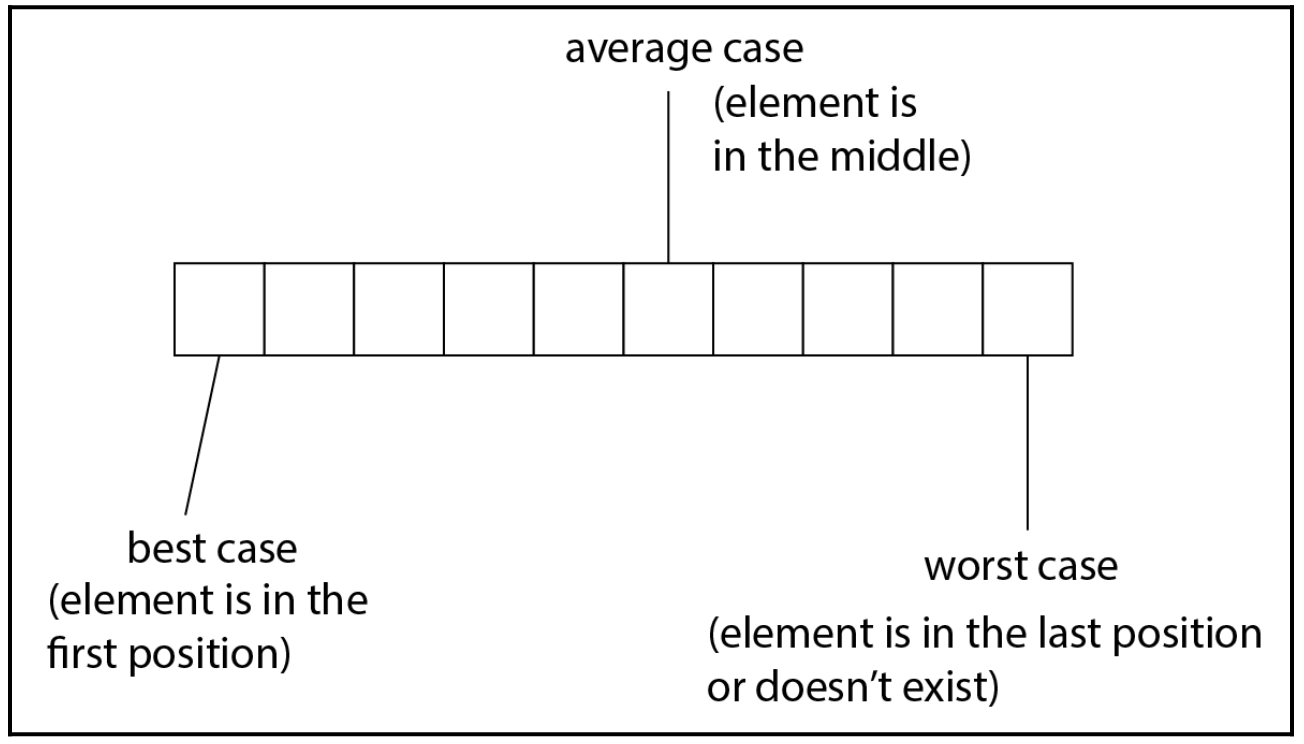
\includegraphics[width=0.6\textwidth]{content/Section-2/Chapter-6/20}
\end{center}

我们应该考虑最坏的情况,因为它也涵盖了所有其他情况。如果在最坏的情况下定义一个算法的复杂度,我们可以肯定其他情况不会比这更慢。 \par
要找出一个算法的复杂性,我们应该找到操作的数量和输入的大小之间的联系。本例中,输入的大小就是容器的长度。我们用A表示拷贝,用C表示比较,用I表示递增操作,这样我们就有$3A + (2n + 1)C + (n + 1)I$个操作。算法的复杂度定义如下: \par 

$O(3A + (2n + 1)C + (n + 1)I)$

这可以通过以下方式简化: \par

\begin{itemize}
	\item $O(3A + (2n + 1)C + (n + 1)I) =$
	\item $O(3A + 2nC + C + nI + I) =$
	\item $O(n(2C + I) + (3A + C + I)) =$
	\item $O(n(2C + I))$
\end{itemize}

最后,O()的属性要去掉常系数和较小的成员,因为实际算法的复杂性只与输入的大小n有关,所以得到最终的复杂性等于O(n)。换句话说,顺序搜索算法的时间复杂度是线性的。 \par
如前所述,STL的本质是通过迭代器连接容器和算法。这就是为什么顺序搜索实现不兼容STL:因为它对输入参数有严格的限制。为了使它泛型,我们应该考虑使用迭代器来实现它。要覆盖更广泛的容器类型,请使用前向迭代器。下面的代码使用Iter类型的操作符,假设它是前向迭代器: \par

\begin{lstlisting}[caption={}]
template <typename Iter, typename T>
int search(Iter first, Iter last, const T& elem)
{
	for (std::size_t count = 0; first != last; first++, ++count) {
		if (*first == elem) return count;
	}
	return -1;
}
...
std::vector<int> vec{4, 5, 6, 7, 8};
std::list<double> lst{1.1, 2.2, 3.3, 4.4};
std::cout << search(vec.begin(), vec.end(), 5);
std::cout << search(lst.begin(), lst.end(), 5.5);
\end{lstlisting}

实际上,任何类型的迭代器都可以传递给search()函数。通过对迭代器本身应用操作,确保使用前向迭代器。我们只使用前向迭代器支持的自增(向前移动)、读(*操作符)和严格比较(==和!=)。 \par

\noindent\textbf{}\ \par
\textbf{二分搜索} \ \par
二分搜索算法很容易解释。首先,寻找向量的中间元素,并与搜索键进行比较,如果它等,那么算法就完成了:它返回索引。否则,如果搜索键小于中间的元素,它将继续到向量的左边。如果搜索键大于中间元素,则算法继续搜索右边的子向量。 \par
为了使二分搜索对一个向量正确工作,它应该排序。二分查找的本质是将搜索键与向量元素进行比较,然后继续查找左边或右边的子向量,与向量的中间元素相比,每个子向量都包含一个更小或更大的元素。看看下面的图表,它描述了二进制搜索算法的运行: \par

\begin{center}
	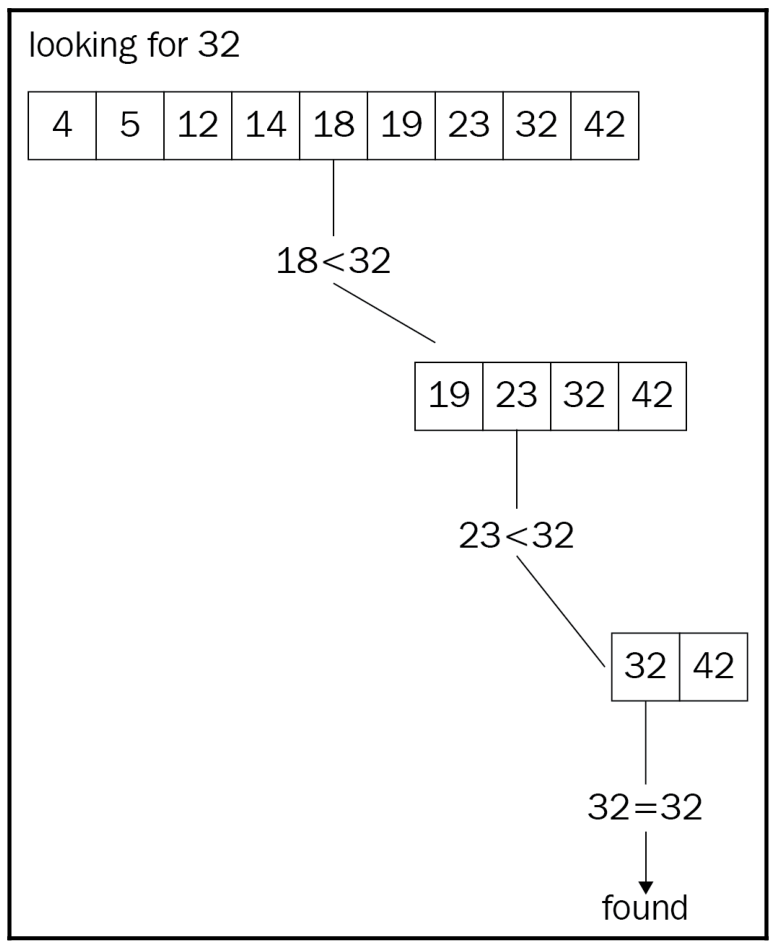
\includegraphics[width=0.4\textwidth]{content/Section-2/Chapter-6/21}
\end{center}

二分搜索算法有一个优雅的递归实现(尽管使用迭代实现更好): \par

\begin{lstlisting}[caption={}]
template <typename T>
std::size_t binsearch(const std::vector<T>& vec, const T& item, int start,
int end)
{
	if (start > end) return -1;
	int mid = start + (end - start) / 2;
	if (vec[mid] == item) {
		return mid; // found
	}
	if (vec[mid] > item) {
		return binsearch(vec, item, start, mid - 1);
	}
	return binsearch(vec, item, mid + 1, end);
}
\end{lstlisting}

注意中间元素的计算。而不是\texttt{(start + end) / 2;},我们使用\texttt{start + (end - start) / 2;}技术只是为了避免二分搜索实现中的bug(假设我们没有留下其他bug)。关键是,对于较大的start和end值,它们的和(start + end)将产生整数溢出,这将使程序在某个点崩溃。 \par
现在来算一下二分搜索的复杂度。执行的每一步中,源数组都减半,所以在下一步中处理它的大小一半,最坏的情况是对向量进行除法,直到剩下一个元素或一个元素都没有。为了求出算法中的步数,我们应该求出与向量大小有关的除法次数。如果向量有10个元素,则除以它,得到一个包含5个元素的子向量。再除以一次,就得到了两个元素的子向量,最后再除以一次,就得到了一个元素。所以,对于10个元素的向量,划分的次数是3。对于有n个元素的向量,划分的次数是log(n),因为在每一步上,n变成n/2,然后变成n/4,以此类推。二分搜索的复杂度是O(logn)(即对数)。 \par
STL算法定义在<algorithm>头文件中,二分搜索的实现驻留在那里。如果元素在容器中存在,则STL实现返回true。看看它的原型: \par

\begin{lstlisting}[caption={}]
template <typename Iter, typename T>
bool binary_search(Iter start, Iter end, const T& elem);
\end{lstlisting}

STL算法不直接与容器一起工作,而是与迭代器一起。这允许我们从特定的容器进行抽象,并对所有支持前向迭代器的容器使用binary\underline{ }search()。下面的例子调用binary\underline{ }search()函数来处理vector和list: \par

\begin{lstlisting}[caption={}]
#include <vector>
#include <list>
#include <algorithm>
...
std::vector<int> vec{1, 2, 3, 4, 5};
std::list<int> lst{1, 2, 3, 4};
binary_search(vec.begin(), vec.end(), 8);
binary_search(lst.begin(), lst.end(), 3);
\end{lstlisting}

binary\underline{ }search()检查迭代器的类别,在随机访问迭代器的情况下,它使用二分搜索算法的全部功能(否则,它将退回到顺序搜索)。 \par

\noindent\textbf{}\ \par
\textbf{排序} \ \par
二分搜索算法只适用于已排序的容器。排序对于计算机程序员来说是一项古老的任务,现在很少编写自己的排序算法实现。有的开发者可能多次使用过std::sort(),而根本不了解它的实现。基本上,排序算法接受一个集合作为输入,并返回一个新的排序过的集合(按照算法用户定义的顺序)。 \par
在许多排序算法中,最流行的(甚至是最快的)是快速排序。任何排序算法的基本思想都是找到更小(或更大)的元素,并与更大(或更小)的元素交换它们,直到整个集合排序完毕。例如,选择排序逻辑上将集合分为两部分,排序和未排序,排序的子数组最初是空的,如下所示: \par

\begin{center}
	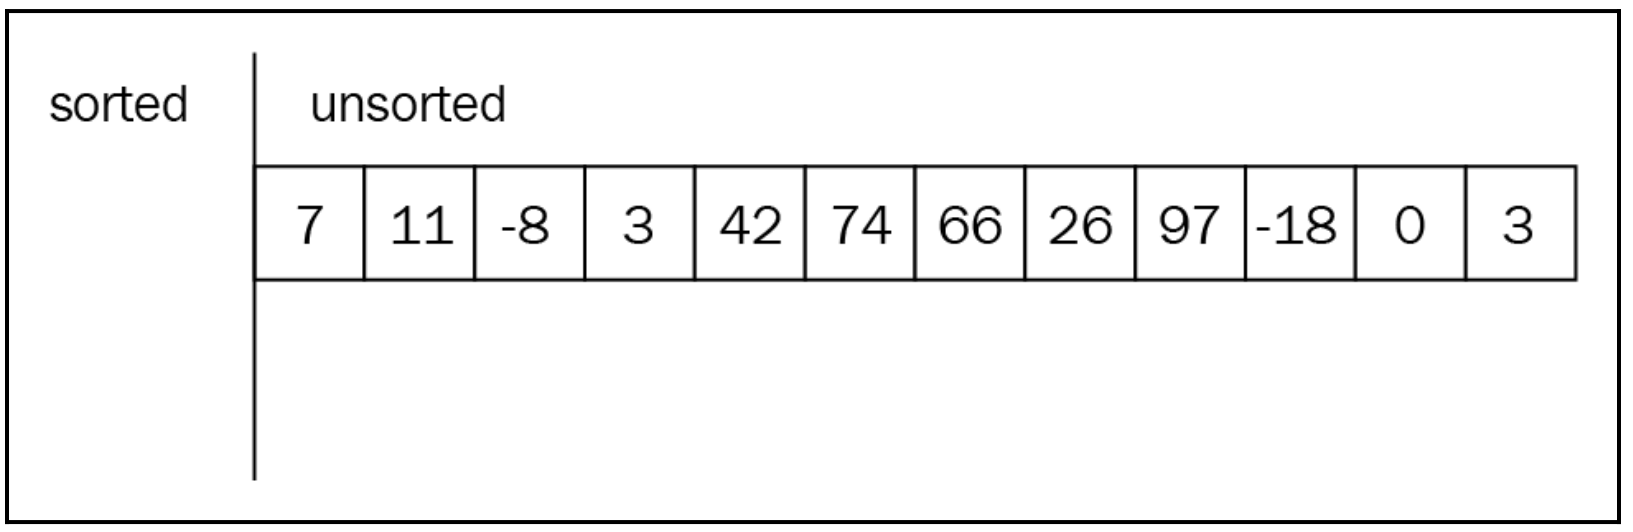
\includegraphics[width=0.6\textwidth]{content/Section-2/Chapter-6/22}
\end{center}

该算法开始在未排序子数组中寻找最小的元素,并通过与未排序子数组的第一个元素交换将其放入已排序子数组中。每一步之后,已排序子数组的长度增加1,而未排序子数组的长度减少如下: \par

\begin{center}
	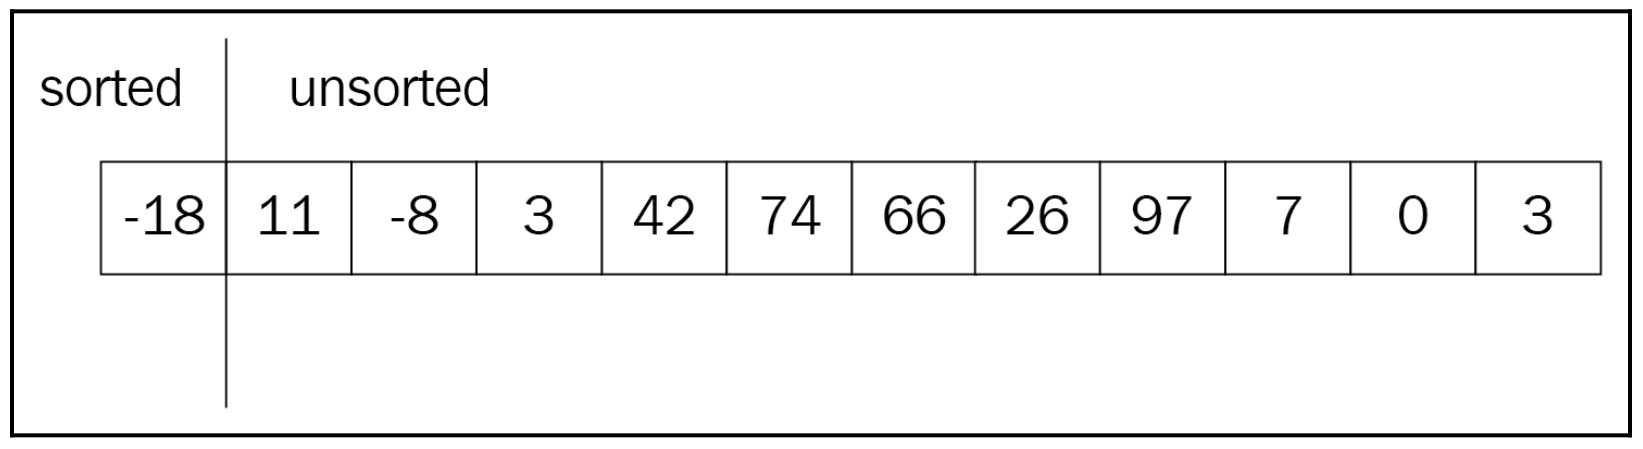
\includegraphics[width=0.6\textwidth]{content/Section-2/Chapter-6/23}
\end{center}

这个过程将继续,直到未排序的子数组变为空。 \par
STL提供了std::sort()函数,接受两个随机访问迭代器: \par

\begin{lstlisting}[caption={}]
#include <vector>
#include <algorithm>
...
std::vector<int> vec{4, 7, -1, 2, 0, 5};
std::sort(vec.begin(), vec.end());
// -1, 0, 2, 4, 5, 7
\end{lstlisting}

sort函数不能应用于std::list,因为它不支持随机访问迭代器,而list应该调用sort()成员函数。尽管这与STL拥有通用函数的想法相矛盾,但这样做是为了提高效率。 \par
sort()函数有第三个形参:一个比较函数,可用于比较容器元素。假设将Product对象存储在vector中: \par

\begin{lstlisting}[caption={}]
struct Product
{
	int price;
	bool available;
	std::string title;
};

std::vector<Product> products;
products.push_back({5, false, "Product 1"});
products.push_back({12, true, "Product 2"});
\end{lstlisting}

要对容器进行正确的排序,容器中的元素必须支持小于操作符。我们应该为自定义类型定义相应的运算符。但是,如果为自定义类型创建单独的比较器函数,则可以省略运算符定义,如下面的代码块所示: \par

\begin{lstlisting}[caption={}]
class ProductComparator
{
	public:
	bool operator()(const Product& a, const Product& b) {
		return a.price > b.price;
	}
};
\end{lstlisting}

将ProductComparator传递给std::sort()函数,允许它比较vector元素,而无需深入了解元素的类型细节,如下所示: \par

\begin{lstlisting}[caption={}]
std::sort(products.begin(), products.end(), ProductComparator{});
\end{lstlisting}

虽然这是一种很好的技术,但使用lambda函数会更优雅,lambda函数是一种匿名函数,非常适合前一种情况。下面是我们使用lambda对sort重新实现: \par

\begin{lstlisting}[caption={}]
std::sort(products.begin(), products.end(),
	[](const Product& a, const Product& b) { return a.price > b.price; })
\end{lstlisting}

上面的代码允许省略ProductComparator的声明。 \par

\noindent\textbf{}\ \par
\textbf{搜索树和图} \ \par
二分搜索算法和排序算法结合在一起,就产生了使用一个容器来默认保存条目排序的想法,其中一个容器std::set就是基于平衡树的。讨论平衡树本身之前,我们先看看二叉搜索树,它是快速查找的最佳选择。 \par
二叉搜索树的思想是一个节点左子树的值小于该节点的值。相比之下,一个节点的右子树的值大于该节点的值。这里有一个二叉搜索树的例子: \par

\begin{center}
	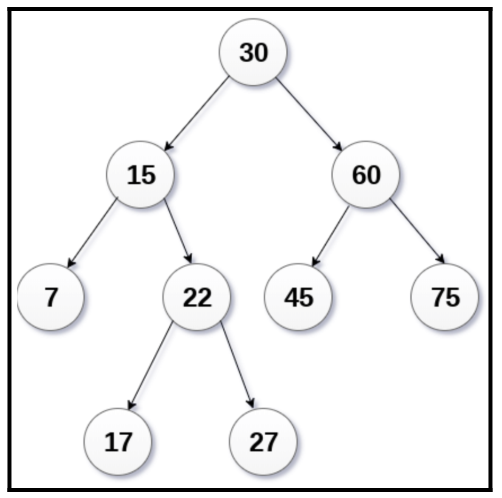
\includegraphics[width=0.4\textwidth]{content/Section-2/Chapter-6/24}
\end{center}

正如图表中看到的,值为15的元素驻留在左边的子树中,因为它小于30(根元素)。另一方面,值为60的元素驻留在右边的子树中,因为它比根元素大。同样的逻辑也适用于其余的树元素。 \par
二叉树节点表示为一个结构体,其中包含项目和指向每个子节点的两个指针。下面是一个表示树节点的示例代码: \par

\begin{lstlisting}[caption={}]
template <typename T>
struct tree_node
{
	T item;
	tree_node<T>* left;
	tree_node<T>* right;
};
\end{lstlisting}

一个完全平衡的二叉搜索树中,搜索、插入或删除一个元素需要O(logn)。STL没有为树提供单独的容器,但是它有类似的基于树实现的容器。例如,std::set容器基于一棵按排序顺序存储元素的平衡树: \par

\begin{lstlisting}[caption={}]
#include <set>
...
std::set<int> s{1, 5, 2, 4, 4, 4, 3};
// s has {1, 2, 3, 4, 5}
\end{lstlisting}

std::map也是基于平衡树的,但它提供了一个容器,将一个键映射到某个值,如下所示: \par

\begin{lstlisting}[caption={}]
#include <map>
...
std::map<int, std::string> numbers;
numbers[3] = "three";
numbers[4] = "four";
...
\end{lstlisting}

如上述代码所示,map将数字映射为字符串。因此,当我们告诉map将值3存储为键值,将字符串“three”存储为值时,它会在其内部树中添加一个新节点,键值为3,值为“three”。 \par
set和map操作是对数的,这使得它在大多数情况下是一个非常高效的数据结构。然而,接下来会出现一个更高效的数据结构。 \par

\noindent\textbf{}\ \par
\textbf{哈希表} \ \par
哈希表是最快的数据结构,基于矢量索引的简单思想。想象一个包含指向列表指针的大向量: \par

\begin{lstlisting}[caption={}]
std::vector<std::list<T> > hash_table;
\end{lstlisting}

访问vector元素需要常量时间。这是向量的主要优势。哈希表允许我们使用任何类型作为容器的键。哈希表的基本思想是使用经过良好管理的哈希函数,该函数将为输入键生成唯一的索引。例如,当使用字符串作为哈希表的键时,哈希表使用函数生成哈希值作为基础向量的索引值: \par

\begin{lstlisting}[caption={}]
template <typename T>
int hash(const T& key)
{
	// generate and return and efficient
	// hash value from key based on the key's type
}
template <typename T, typename U>
void insert_into_hashtable(const T& key, const U& value)
{
	int index = hash(key);
	hash_table[index].push_back(value); // insert into the list
}
\end{lstlisting}

下面是如何使用哈希表: \par

\begin{center}
	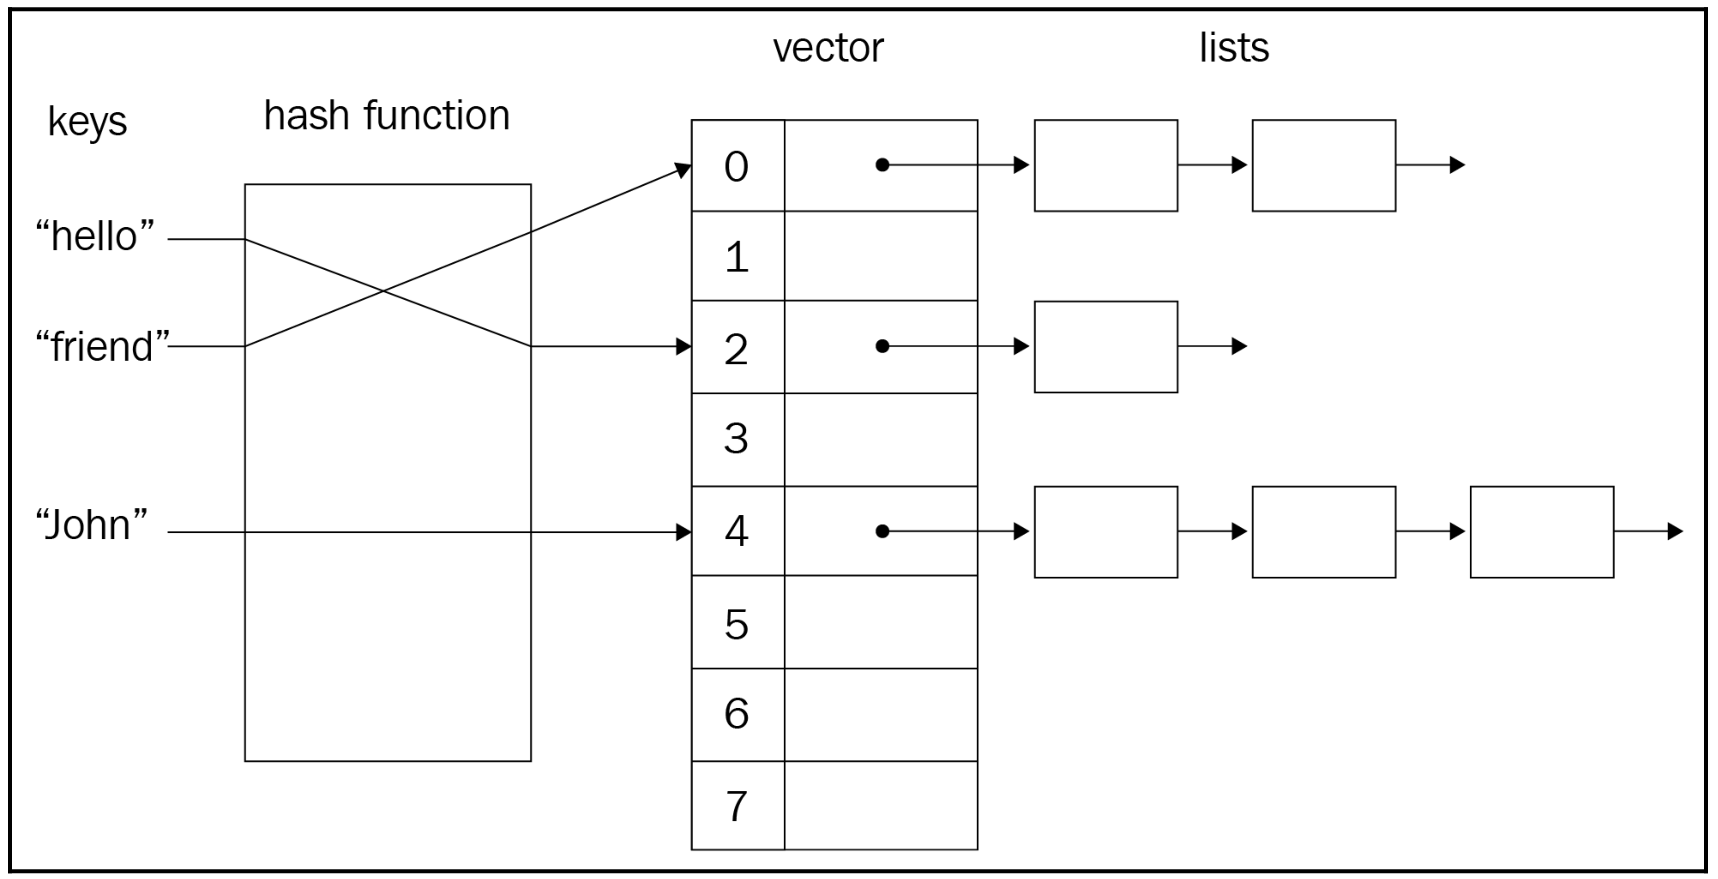
\includegraphics[width=0.6\textwidth]{content/Section-2/Chapter-6/25}
\end{center}

访问哈希表需要常量时间,因为它基于vector操作。虽然可能有不同的键会导致相同的散列值,但是这些冲突可以通过使用一个值列表作为vector元素来解决(如上图所示)。 \par
STL支持一个名为std::unordered\underline{ }map的哈希表: \par

\begin{lstlisting}[caption={}]
#include <unordered_map>
...
std::unordered_map<std::string, std::string> hashtable;
hashtable["key1"] = "value 1";
hashtable["key2"] = "value 2";
...
\end{lstlisting}

要为提供的键生成散列值,函数std::unordered\underline{ }map使用<functional>头文件中定义的std::hash()函数。可以为哈希函数指定自定义实现。std::unordered\underline{ }map的第三个模板参数是散列函数,默认为std::hash。 \par

\noindent\textbf{}\ \par
\textbf{图} \ \par
二叉搜索树的平衡特性基于多种搜索索引实现。例如,数据库系统使用一种称为B-树的平衡树来索引表。B-树不是二叉树,但遵循相同的平衡逻辑,如下图所示: \par

\begin{center}
	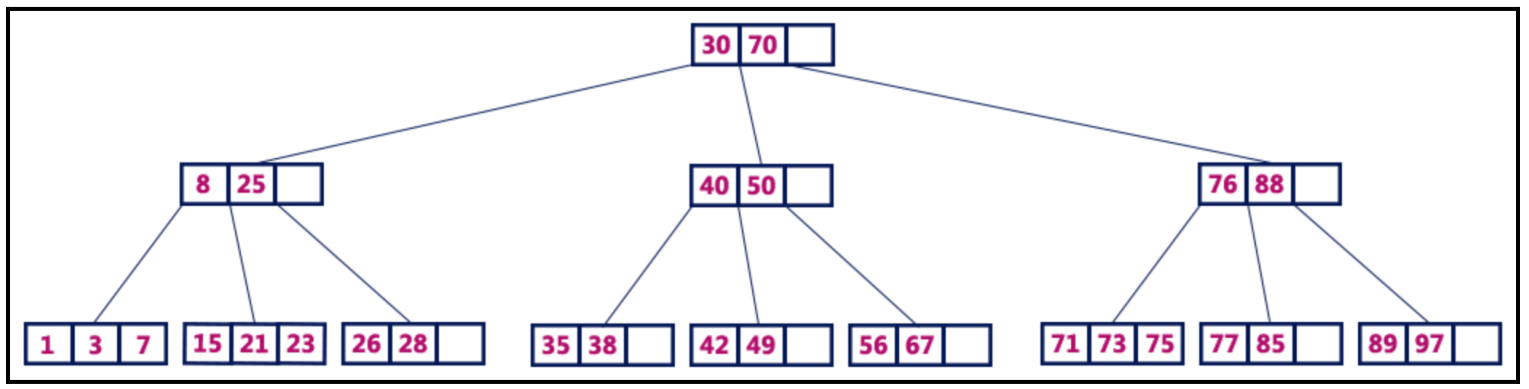
\includegraphics[width=0.6\textwidth]{content/Section-2/Chapter-6/26}
\end{center}

另一方面,图表示节点间的连接: \par

\begin{center}
	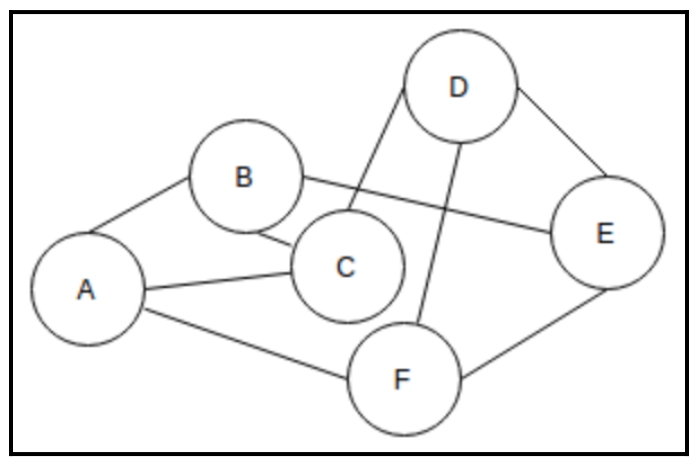
\includegraphics[width=0.4\textwidth]{content/Section-2/Chapter-6/27}
\end{center}

假设正在建立一个最终会在市场上击败Facebook的社交网络。社交网络中的用户可以互相关注,可以用图表来表示。例如,如果A遵循B, B遵循C,并且C同时遵循B和A,那么我们可以将这些关系表示为如下图: \par

\begin{center}
	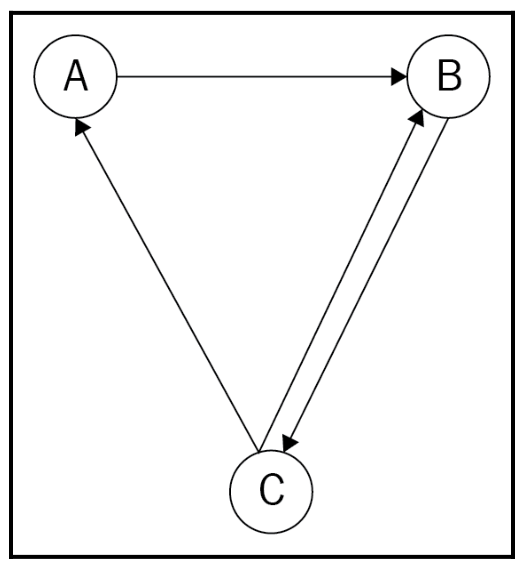
\includegraphics[width=0.4\textwidth]{content/Section-2/Chapter-6/28}
\end{center}

一个节点称为图中的一个顶点。两个节点之间的连接称为边。实际上并没有一个固定的图表示,所以我们应该从几个图中选择一个。想想我们的社交网络——我们如何表示用户A关注用户B的信息? \par
最好的选择之一是使用哈希表,可以将用户与他们关注的所有用户进行映射: \par

\begin{center}
	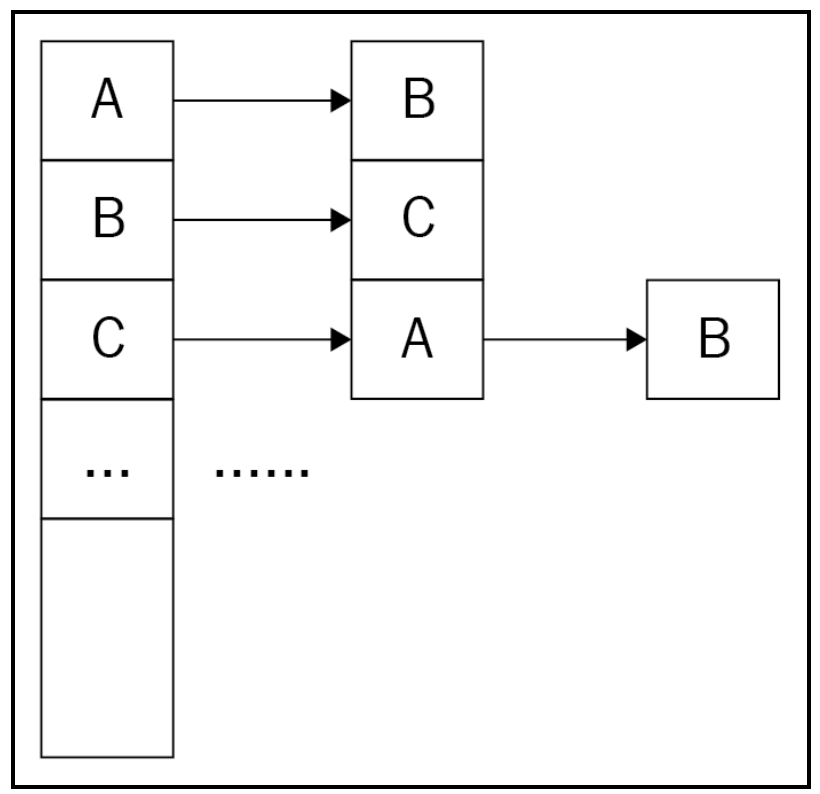
\includegraphics[width=0.4\textwidth]{content/Section-2/Chapter-6/29}
\end{center}

图实现变成了一个混合容器: \par

\begin{lstlisting}[caption={}]
#include <list>
#include <unordered_map>
template <typename T>
class Graph
{
public:
	Graph();
	~Graph();
	// copy, move constructors and assignment operators omitted for brevity
	
public:
	void insert_edge(const T& source, const T& target);
	void remove_edge(const T& source, const T& target);
	
	bool connected(const T& source, const T& target);
	
private:
	std::unordered_map<T, std::list<T> > hashtable_;
};
\end{lstlisting}

为了创建一个与STL兼容的容器,为图添加一个迭代器。虽然迭代一个图不是个好主意,但是添加一个迭代器也不是个坏主意。 \par

\noindent\textbf{}\ \par
\textbf{字符串} \ \par
字符串类似于vector:它们存储字符,具有迭代器,还是容器。然而,字符串则有些不同。下面的图表将字符串“hello, C++”描述为一个以特殊$\backslash$0字符结尾的字符数组: \par

\begin{center}
	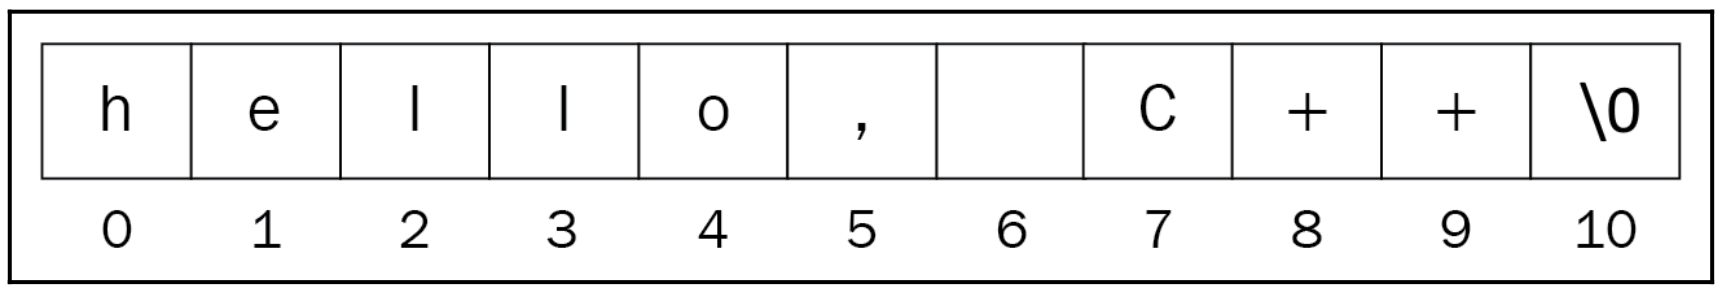
\includegraphics[width=0.6\textwidth]{content/Section-2/Chapter-6/30}
\end{center}

特殊的$\backslash$0字符(也称为空字符)用作字符串终止符。编译器一个接一个地读取字符,直到遇到空字符。 \par
string对象的实现方式与本章开头vector对象的实现方式相同: \par

\begin{lstlisting}[caption={}]
class my_string
{
public:
	my_string();
	// code omitted for brevity
public:
	void insert(char ch);
	// code omitted for brevity
private:
	char* buffer_;
	int size_;
	int capacity_;
};
\end{lstlisting}

C++有强大的std::string类,它提供了一组可以使用的函数。除了std::string的成员函数之外,<algorithm>中定义的算法也适用于字符串。 \par

\noindent\textbf{}\ \par
\textbf{总结} \ \par
数据结构和算法是开发高效软件的关键。通过理解和利用本章讨论的数据结构,你将掌握C++20的全部功能,并且使你的程序运行得更快。有很强的问题解决能力的开发者在市场上更受欢迎,这不是什么秘密。解决问题的技巧首先要通过对基本算法和数据结构的深刻理解来获得。正如在本章中看到的,在搜索任务中使用二分搜索算法使代码运行得比顺序搜索算法快得多。高效的软件可以节省时间并提供更好的用户体验,这最终会使你的软件成为现有软件的杰出替代品。 \par
本章中,我们讨论了基本的数据结构及其区别,通过问题分析学会了使用它们。例如,由于list元素访问操作的复杂性,在需要随机查找的问题中应用list是不合适的。在这种情况下,使用动态增长的向量更合适,因为它的元素访问时间是常量。相反,在需要在容器前端进行快速插入的问题中,使用vector的成本比使用list的成本更高。 \par
本章还介绍了它们效率的度量算法和方法。我们比较了几个问题,以应用更好的算法来更有效地解决它们。 \par
下一章中,我们将讨论C++中的函数式编程。学习了STL的要点之后,我们现在要在容器上应用函数式编程技术了。 \par

\noindent\textbf{}\ \par
\textbf{问题} \ \par
\begin{enumerate}
	\item 描述将元素插入动态增长向量的过程。
	\item 在链表的前面插入元素和在vector的前面插入元素有什么区别?
	\item 实现一个混合数据结构,将其元素存储在vector和list中。对于每个操作,选择具有最快实现该操作的底层数据结构。
	\item 如果我们按递增顺序插入100个元素,那么二叉搜索树会是什么样子呢?
	\item 选择排序和插入排序算法有什么区别?
	\item 实现本章中描述的排序算法,称为计数排序。
\end{enumerate}

\noindent\textbf{}\ \par
\textbf{扩展阅读} \ \par
有关更多信息,请参阅以下参考资料: \par

\begin{itemize}
	\item Programming Pearls by Jon Bentley, available from  https:/​/​www.​amazon.​com/	Programming-​Pearls-​2nd-​Jon-​Bentley/​dp/​0201657880/​
	\item Data Abstraction and Problem Solving Using C++: Walls and Mirrors by Frank Carrano,and Timothy Henry, available from  https:/​/​www.​amazon.​com/​Data-Abstraction-​Problem-​Solving-​Mirrors/​dp/​0134463978/​
	\item Introduction to Algorithms by Cormen, Leiserson, Rivest, and Stein, available
	from https:/​/​www.​amazon.​com/​Introduction-​Algorithms-​3rd-​MIT-​Press/​dp/0262033844/​
	\item C++ Data Structures and Algorithms by Wisnu Anggoro, available from  https:/​/
	www.​packtpub.​com/​application-​development/​c-​data-​structures-​and-algorithms
\end{itemize}

\newpage







